%% ------------------- LICENSE ---------------------%%
%% --------------------------------------------------%%
%% Universidad Distrital Francisco Jose de Caldas
%% Revista Tecnura
%%https://revistas.udistrital.edu.co/ojs/index.php/Tecnura/issue/view/1033
%% Bogota, Colombia
%%Template creado por Julian Arcila-Forero, M.Sc.
%%jfarcilaf@udistrital.edu.co
%%Centro de Investigaciones y Desarrollo Científico - UDFJC
%%Abril, 2025
%%Modificada bajo las condiciones del LaTeX Project Public License http://www.latex-project.org/lppl.txt.
%% ------------------------------------------------------%%
\PassOptionsToPackage{table,xcdraw}{xcolor}
\documentclass[letterpaper,11pt]{tec}

\usepackage[pdfauthor={Edier Aristizábal},
            pdftitle={Implementación de Procesos Gaussianos para la evaluación de la susceptibilidad por movimientos en masa},
            pdfsubject={https://doi.org/10.14483/22487638.xxxxx},
            pdfkeywords={susceptibilidad, movimientos en masa, procesos gaussianos, incertidumbre, aprendizaje automático, Colombia},
            pdfproducer={Latex with hyperref},
            pdfcreator={Oficina de Investigaciones,  revistas-cidc@udistrital.edu.co}, backref=page]{hyperref}
%%%%%%%%%%%%%%%
\urlstyle{same}
\hypersetup{colorlinks=true,linkcolor=black,urlcolor=blue1,anchorcolor=black,citecolor=blue1}
\renewcommand\UrlFont{\color{blue1}\normalfont}
\usepackage[figurename=Figura]{caption}
\captionsetup{labelfont={color=black,bf}, labelsep=period,font=small}
\usepackage{colortbl}
\arrayrulecolor{gray}
\usepackage{booktabs}
\usepackage{nicefrac}
\usepackage{array}
\usepackage[numbers]{natbib}
\graphicspath{{FIGURAS/}}
\setlength{\headheight}{75pt}

\begin{document}


%%------------------TITULO -------------------%%
%%--------------------------------------------%%
\vspace{1.15cm}
\rightline{\color{gray}\normalsize \bf INVESTIGACIÓN}
\vspace{1cm}
\begin{center}
{\fontencoding{T1}\fontfamily{}\fontseries{b}\fontshape{n}
\fontsize{16}{17}\selectfont\bf
Implementación de Procesos Gaussianos para la evaluación de la susceptibilidad por movimientos en masa}\vspace{0.15cm}
\end{center}
\begin{center}
{\color{gray} \Large\bf
Implementation of Gaussian Processes for Landslide Susceptibility Assessment}\end{center}

%% --------------------- AUTORES --------------------- %%
%% --------------------------------------------------- %%
\begin{center}
%---------------------------------------------------------------------------




%---------------------------------------------------------------------------
Edier Aristizábal\href{https://orcid.org/0000-0002-2648-2197}{
\includegraphics[scale=0.065]{orcid.jpeg}}\footnote{Ingeniero geólogo con especialización en Gestión del Riesgo y Desastres asociados al Clima de la Universidad de Ginebra, Suiza; Maestría en Geociencias de la Universidad de Shimane, Japón; Doctor en Ingeniería de la Universidad Nacional de Colombia; Posdoctorado de la Universidad de Potsdam, Alemania. Actualmente profesor del Departamento de Geociencias y Medio Ambiente, Universidad Nacional de Colombia, sede Medellín.\href{https://ror.org/059yx9a68}{
\includegraphics[scale=0.025]{ror.png}}.   Email:
{\color{blue1}evaristizabalg@unal.edu.co}}
\end{center}


%% --------------------- CITACION --------------------- %%
%% ---------------------------------------------------- %%
\setlength{\columnsep}{1.5cm}
\begin{multicols}{2}
\noindent { \small {\bf Fecha de Recepción}: xx de xxxxxx de 202x\\
{\bf Fecha de Aceptación}: xx de xxxxxx de 202x}
\end{multicols}
\vspace{0.1cm}
\begin{tcolorbox}
[colback=gray!10!white,colframe=white!65!white,fonttitle=\bfseries,]{\color{black}{ \bf Cómo citar}}:
\small E. Aristizábal, ``Implementación de Procesos Gaussianos para la evaluación de la susceptibilidad por movimientos en masa,'' {\it Tecnura}, vol. xx, no. xx, pp. xx--xx, 202x, {\color{tinto}\href{https://doi.org/10.14483/22487638.xxxxx}{https://doi.org/10.14483/22487638.xxxxx}}
\end{tcolorbox}




%% ------------------ RESUMEN Y ABSTRACT ------------------ %%
%% -------------------------------------------------------- %%

\renewcommand{\baselinestretch}{1.25}
\vspace{-0.5cm}
\footnotesize{




\section*{\color{black}Resumen}
\noindent{\bf Objetivo:} Evaluar la susceptibilidad por movimientos en masa en la cuenca La Iguana
(52{,}2~km$^2$, Medellín, Colombia) mediante un marco secuencial de Procesos Gaussianos de Regresión (PGR)
y Clasificación (PGC).
\\\noindent{\bf Metodología:} Se implementó un PGR entrenado sobre la superficie de densidad del inventario
(583 eventos, estimación por kernel con ancho de banda de Silverman $\approx$~691~m) y un PGC binario con
verosimilitud de Bernoulli e inferencia por aproximación de Laplace, ambos con función de covarianza
Matérn-$\nicefrac{3}{2}$ y Determinación Automática de Relevancia (ARD). Se evaluaron cuatro combinaciones de
variables condicionantes sobre las 2{,}087{,}643 celdas de la cuenca a resolución de 5~m.
\\\noindent{\bf Resultados:} El PGR no discriminó adecuadamente los sitios susceptibles (AUC~=~0{,}559).
El PGC con tres variables ---pendiente, geología y cobertura del suelo--- alcanzó AUC~=~0{,}823,
prácticamente idéntico al \textit{Benchmark} de cinco variables (AUC~=~0{,}826). El análisis ARD revela la
dominancia de la cobertura del suelo (importancia~0{,}272), seguida de la pendiente (0{,}215) y la
geología (0{,}062).
\\\noindent{\bf Conclusiones:} El PGC es estadísticamente más apropiado para la cartografía de susceptibilidad
a escala de celda. El mapa de desviación estándar posterior identifica objetivamente las zonas pobremente
restringidas por los datos históricos, diferenciando zonas prioritarias para mitigación de aquellas que
demandan datos adicionales de campo.
\\\noindent{\bf Financiamiento:} Esta investigación no recibió financiamiento externo.
\\

\noindent\textbf{\textit{Palabras clave:}} susceptibilidad, movimientos en masa, procesos gaussianos, incertidumbre, aprendizaje automático, Colombia.




{\color{gray}\hrule height 0.035cm}




\vspace{0.1cm}

\section*{\color{black}Abstract}
\noindent{\bf Objective:} To evaluate landslide susceptibility in the La Iguana watershed
(52.2~km$^2$, Medellín, Colombia) using a sequential framework of Gaussian Process Regression (GPR)
and Gaussian Process Classification (GPC).
\\\noindent{\bf Methodology:} A GPR was trained on the spatial density of a landslide inventory
(583 events, kernel density estimation with Silverman bandwidth $\approx$~691~m) and a binary GPC
with Bernoulli likelihood and Laplace approximation inference, both using the Matérn-$\nicefrac{3}{2}$
covariance function with Automatic Relevance Determination (ARD). Four combinations of conditioning
variables were evaluated over 2,087,643 cells at 5~m resolution.
\\\noindent\textbf{Results:} The GPR failed to adequately discriminate susceptible sites (AUC~=~0.559).
The GPC with three variables---slope, geology, and land cover---achieved AUC~=~0.823, nearly identical
to the five-variable benchmark (AUC~=~0.826). ARD analysis reveals the dominance of land cover
(importance~0.272), followed by slope (0.215) and geology (0.062).
\\\noindent\textbf{Conclusions:} GPC is statistically more appropriate for cell-scale susceptibility mapping.
The posterior standard deviation map objectively identifies zones poorly constrained by historical data,
distinguishing priority areas for mitigation from those requiring additional field data.
\\\noindent\textbf{Funding:} This research received no external funding.
\\

\noindent\textbf{\textit{Keywords:}} susceptibility, landslides, Gaussian processes, uncertainty, machine learning, Colombia.


{\color{gray}\hrule height 0.05cm}\vspace{0.3cm}
\newpage

%% ----- ENCABEZADO Y PIE DE PAGINA PRIMER PAGINA --------- %%
%% -------------------------------------------------------- %%
\pagestyle{fancy}
\fancyhf{}
\fancyhead[C]{}
\fancyhead[C]{\footnotesize{Implementación de Procesos Gaussianos para la evaluación de la susceptibilidad por movimientos en masa}\\
\vspace{0.1cm}
\scriptsize{E. Aristizábal}\\}
\fancyfoot[C]{\scriptsize{{\bf Tecnura} • p-ISSN: 0123-921X • e-ISSN: 2248-7638 • Volumen xx Número xx • xxxx - xxxx de 202x • pp. xx-xx \\}\normalsize[\thepage]}

%% ---------------CUERPO DEL ARTICULO -------------------- %%
%% ------------------------------------------------------- %%
\normalsize


\vspace{-0.35cm}
\section{Introducción}
\renewcommand{\tablename}{Tabla}
\renewcommand{\figurename}{Figura}

Los movimientos en masa son una de las amenazas de origen natural de mayor recurrencia y afectaciones en terrenos de montaña y
ambientes tropicales \citep{Varnes1978, Hungr2014, Gomez2023}. En Colombia, la confluencia de topografía montañosa, perfiles de meteorización
profunda, lluvias de alta intensidad y expansión urbana acelerada en zonas de ladera crean condiciones de riesgo muy altas
\citep{Aristizabal2012}. La cartografía de susceptibilidad por movimientos en masa estima la probabilidad espacial de falla de uan ladera a partir de las características
del terreno y condiciones ambientales, constituyendo la base para la zonificación del riesgo, la planificación territorial y el diseño 
de medidas de mitigación de riesgo \citep{Guzzetti2005, Corominas2014}. Durante las últimas décadas se ha desarrollado un amplio 
espectro de enfoques estadísticos
y de aprendizaje automático, desde métodos bivariados como Peso de la Evidencia, regresión logística (RL), máquinas de soporte vectorial, bosques
aleatorios y redes neuronales profundas \citep{Reichenbach2018, Chen2017, Corominas2014}. La mayoría de los métodos estadísticos y de 
aprendizaje automático para la cartografía de susceptibilidad por deslizamientos comparten una
arquitectura común: a partir de una muestra de entrenamiento que combina sitios con y sin deslizamientos, el modelo aprende una
regla general que relaciona las características del terreno con la probabilidad de ocurrencia; esa regla se replica luego
uniformemente sobre la totalidad de las unidades del territorio de interés \citep{VanWesten2003, Reichenbach2018}. Esta lógica de modelo global
tiene la ventaja de ser transferible y de no requerir el cómputo explícito de ecuaciones de equilibrio físico. Sin embargo, la
calidad de la regla aprendida depende críticamente de la representatividad del conjunto de entrenamiento y de la capacidad del
modelo para generalizar más allá de los casos observados \citep{Heckmann2014}.

Un aspecto sistemáticamente omitido en la cartografía convencional de susceptibilidad es la cuantificación explícita de la
incertidumbre asociada a cada predicción. La susceptibilidad es inherentemente incierta: los datos de entrada contienen ruido de
medición, el inventario de deslizamientos es incompleto y espacialmente sesgado, y existen variables latentes no observadas, 
profundidad del perfil de meteorización, permeabilidad secundaria, lluvia efectiva, entre otros, cuya influencia sobre la estabilidad de laderas
es significativa pero que generalmente no puede capturarse con las covariables topográficas y ambientales disponibles \citep{Corominas2014}.

La concepción dominante en el modelado de susceptibilidad por deslizamientos trata el problema como una clasificación por unidades de análisis: el
territorio se subdivide en unidades de mapeo, tales como áreas administrativas, cuencas, slope units o celdas de una
cuadrícula, y se asigna un valor escalar de susceptibilidad a cada unidad \citep{Guzzetti2005, Reichenbach2018}. Aunque el uso
de celdas de alta resolución reduce el área de cada unidad, la lógica subyacente no cambia: el valor de cada celda se estima de
forma independiente, sin imponer restricciones de continuidad espacial con sus vecinas. El resultado puede presentar transiciones
abruptas entre celdas adyacentes con condiciones ambientales y topográficas similares, inconsistentes con el carácter continuo y
gradual de los procesos geomorfológicos que controlan la estabilidad de la ladera. Una perspectiva alternativa consiste en tratar la
susceptibilidad como una superficie continua: una función espacialmente coherente que varía de forma suave a través del
paisaje y cuya estructura de correlación refleja la dependencia natural entre sitios próximos \citep{Lombardo2020}.

Los Procesos Gaussianos (PG) ofrecen un marco probabilístico no paramétrico que, de forma natural, responde a los tres desafíos
anteriores \citep{Rasmussen2006}. En términos intuitivos, un PG define una distribución de probabilidad directamente sobre
funciones: en lugar de producir una única estimación de susceptibilidad, el modelo mantiene una familia de funciones compatibles
con los datos observados y, para cualquier localización del territorio, proporciona simultáneamente la susceptibilidad media de las 
funciones compatibles y la incertidumbre de esa estimación expresada como una distribución posterior completa. La estructura de 
correlación espacial está codificada en una función de covarianza, que impone coherencia entre localizaciones próximas y convierte al mapa
predicho en una superficie continua: la información de un punto observado se propaga de forma controlada hacia su entorno,
evitando las transiciones abruptas propias de los modelos por unidades independientes. Los PG pueden emplearse tanto en modo
regresión (PGR), con variable respuesta continua, como en modo clasificación (PGC), con respuesta binaria; y sus aplicaciones
en amenazas naturales incluyen la evaluación del riesgo por deslizamientos en asentamientos de alta montaña mediante GPC
\citep{Gao2021}, la mejora de índices estadísticos de susceptibilidad combinando GPR con análisis de factores espaciales
\citep{Cheng2022}, y el pronóstico probabilístico de series temporales de desplazamiento de laderas con GPR disperso
\citep{Yang2022}. Su principal limitación frente a métodos más ampliamente utilizados, como regresión logística,
bosques aleatorios y redes neuronales, es el elevado costo computacional, que escala cúbicamente con el número de puntos de
entrenamiento ($\mathcal{O}(n^3)$), restringiendo su aplicabilidad directa a muestras de tamaño moderado \citep{Rasmussen2006}.

El Valle de Aburrá en los Andes colombianos, donde se encuentra la ciudad de Medellín, ha registrado
centenares de movimientos en masa con víctimas fatales desde su expansión sobre las laderas a partir de la segunda mitad del siglo XX \citep{Nieto2025, Klimes2010}.
En este artículo se aplica un marco metodológico con Procesos Gaussianos para evaluar la susceptibilidad por movimientos en masa en una cuenca de la ciudad de Medellín, 
considerando la susceptibilidad como una variable continua (densidad de movimientos en masa) o binaria (ocurrencia o no ocurrencia)
 utilizando variables morfométricas continuas y variables ambientales categóricas. Los modelos implementados incorporan la incertidumbre posterior y su relación 
 con el espacio de covariables para identificar zonas que requieren datos adicionales de campo.

\section{Área de estudio}

El área de estudio es la cuenca La Iguana (Fig.~\ref{fig:area_estudio}), ubicada en la vertiente occidental de la Cordillera
Central de los Andes Colombianos, dentro de la unidad geografica conocida como Valle de Aburrá. Con una superficie de 52{,}2~km$^2$ 
y elevaciones entre 1465 y 3141~m~s.n.m. \citep{AristizabalYokota2008}. La cuenca presenta una red de drenaje dendrítica con alta densidad de drenaje
 y un relieve superior a 1500~m, reflejo del encañonamiento fluvial asociado al tectonismo activo de los Andes colombianos
\citep{AristizabalYokota2008, GarciaDelgado2020}.

La geología está dominada por rocas metamorficas, tipo esquistos, anfibolitas y gneis, que constituyen el núcleo metamórfico de la 
Cordillera Central entre las fallas de Otú-Pericos
al oriente y la falla de San Jerónimo al occidente \citep{MayaGonzalez1995, Vinasco2006}. Estas rocas metamórficas están
intensamente fracturadas y meteorizadas, generando perfiles de saprolito de 5 a 20~m de profundidad, susceptibles a deslizamientos
 durante eventos de lluvia \citep{Aristizabal2023}. Estas rocas metamorficas están intruidas localmente por cuerpos graniticos y 
 flanqueado por rocas volcánicas de afinidad oceanica tipo dunitas al norte y basaltos al sur. las laderas del valle estan cubiertas por 
 depositos de vertiente \citep{Garcia2006} y el fondo del valle está cubierto por depósitos aluviales, aluviotorrenicales \citep{MayaGonzalez1995}.

El régimen climático es tropical bimodal, con precipitaciones medias anuales de 1800 a 3000~mm concentradas en dos períodos
lluviosos (marzo--mayo y septiembre--noviembre). Las tormentas convectivas de alta intensidad y corta duración constituyen el
principal detonante de los movimientos en masa en la cuenca \citep{Aristizabal2023}.

\begin{figure}[H]
    \centering
    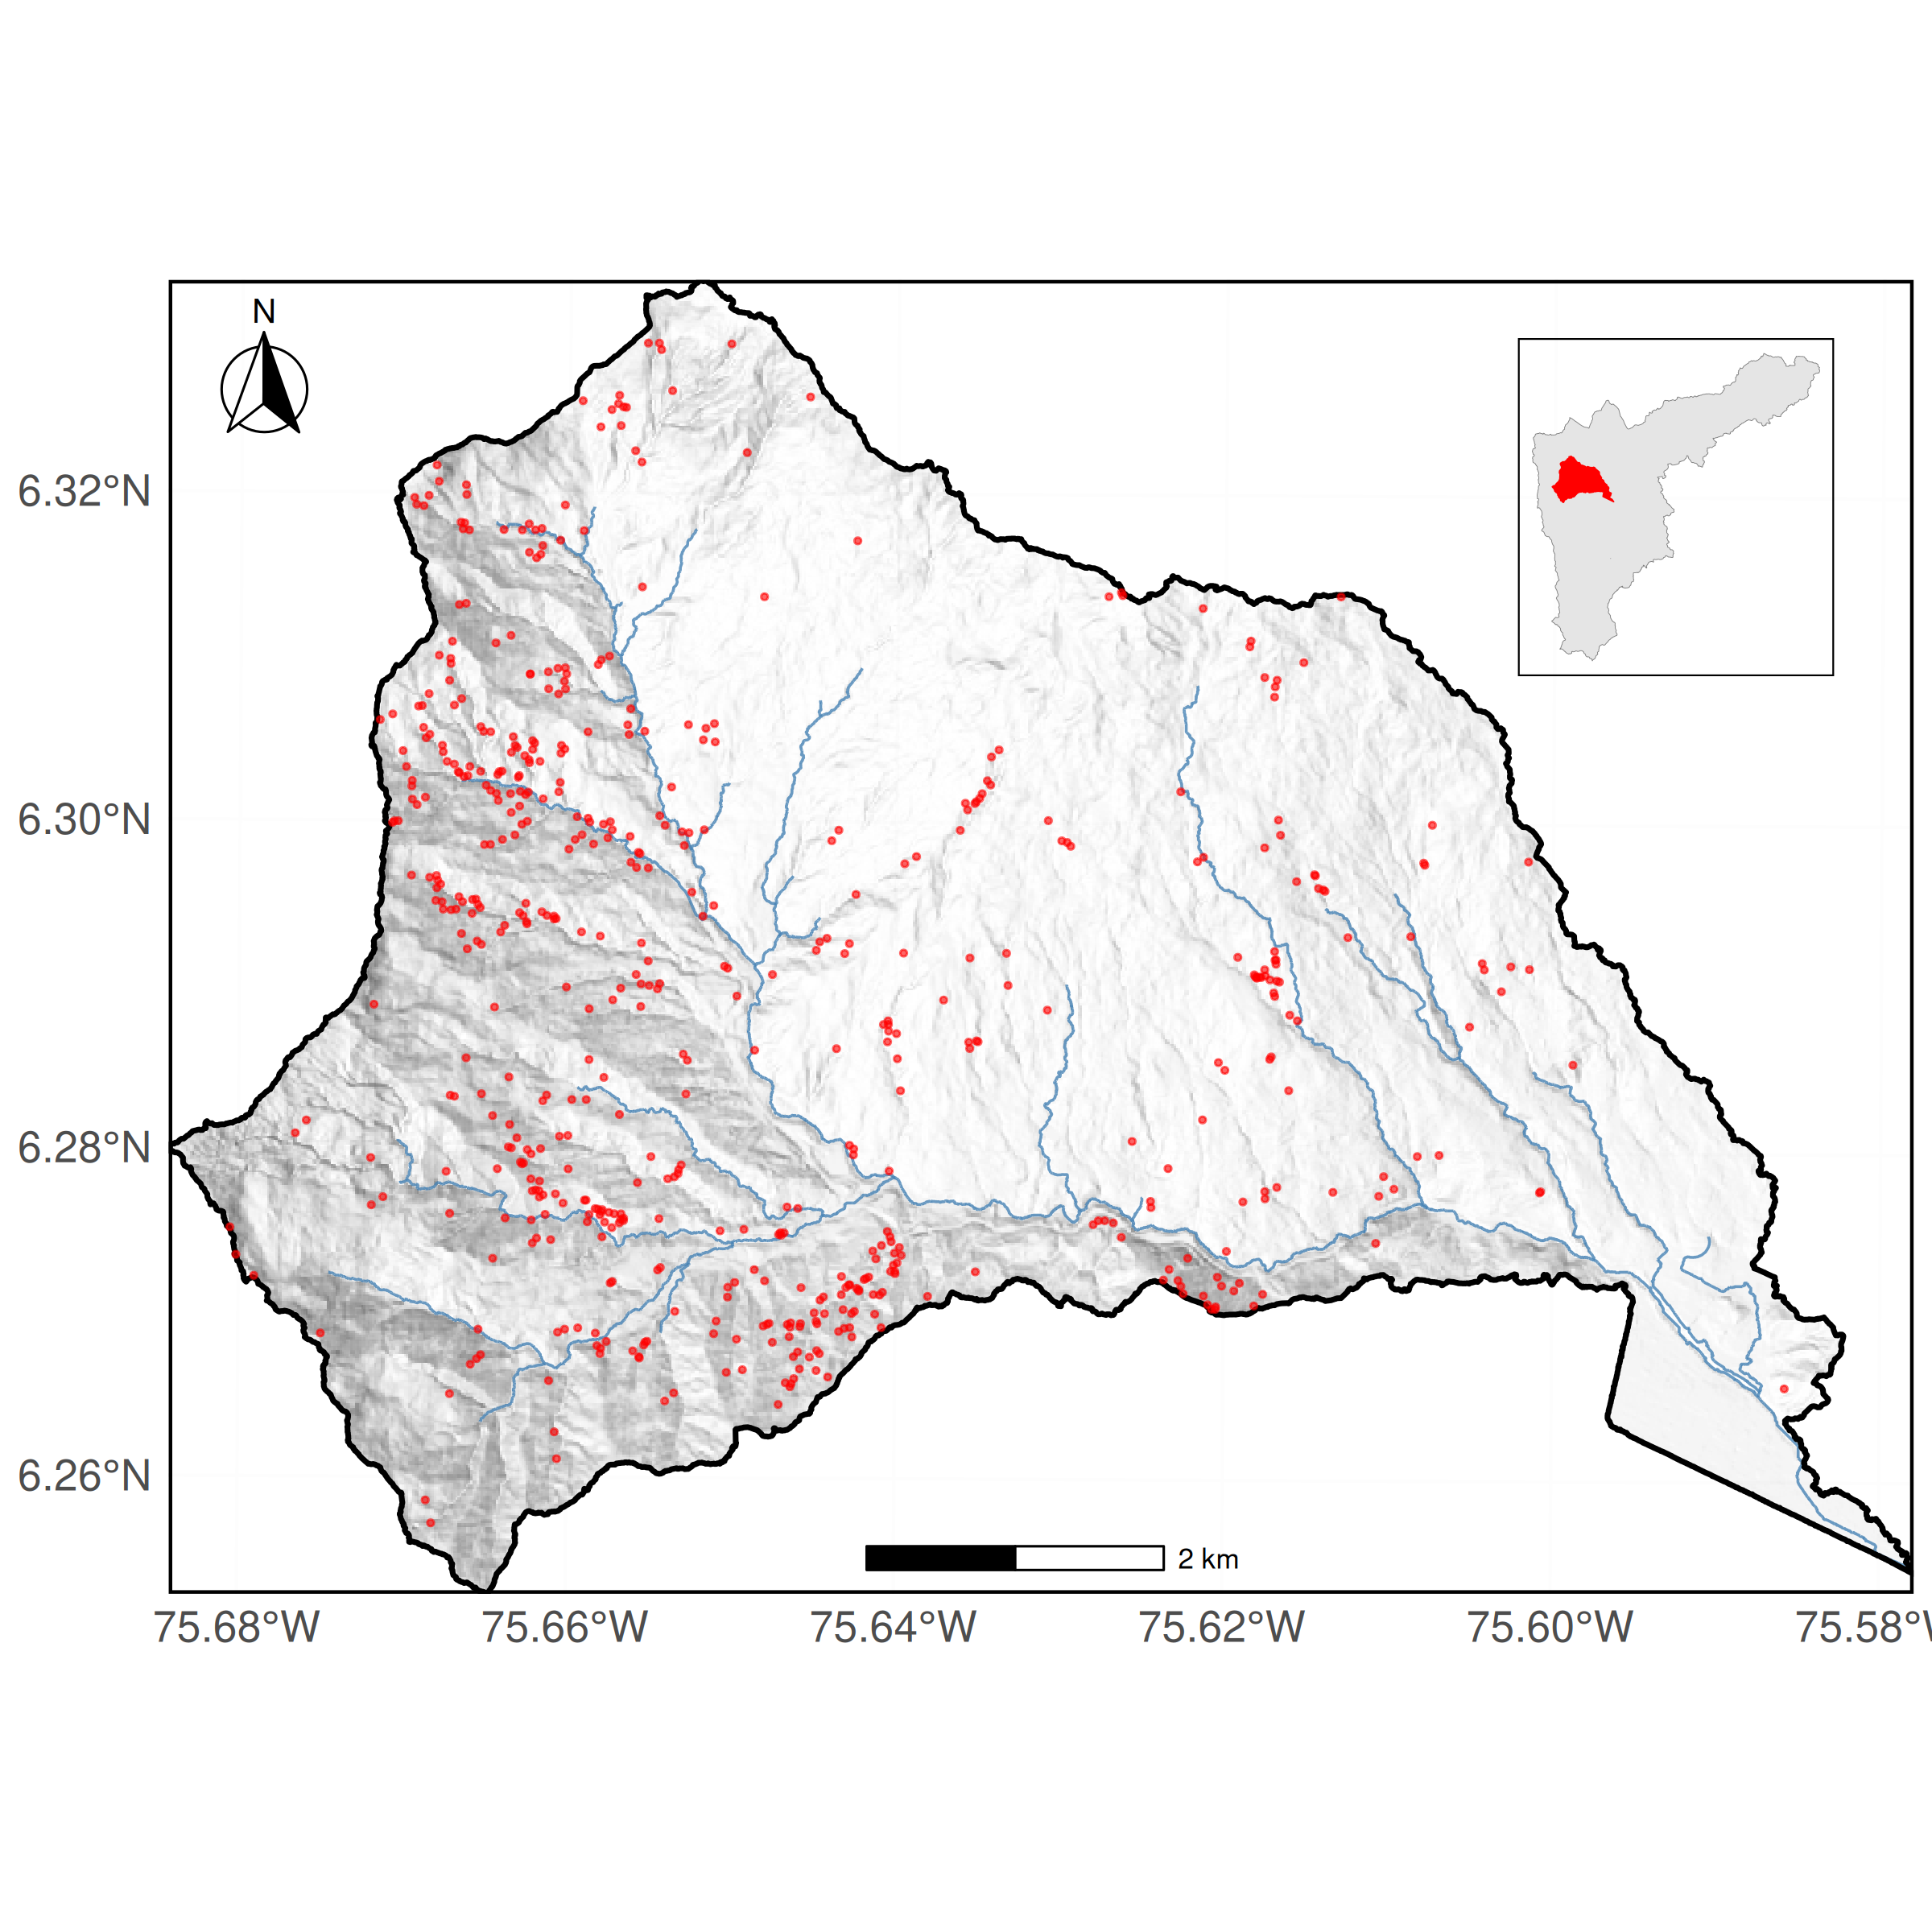
\includegraphics[width=0.85\textwidth]{Fig1_study_area.png}
    \caption{Área de estudio: Cuenca La Iguana. El mapa principal muestra el relieve sombreado con la localización del inventario 
    de movimientos en masa (puntos rojos, $n = 583$) y la red de drenaje. 
    El recuadro muestra la localización regional dentro del Valle de Aburrá.}
    \label{fig:area_estudio}
\end{figure}

\section{Datos y metodología}
\label{sec:metodos}

El inventario de movimientos en masa empleado comprende 583 eventos georreferenciados en la cuenca La Iguaná,
construido mediante interpretación visual sistemática de imágenes de alta resolución submétrica disponibles en Google
Earth para el período 2000--2025. Cada evento fue delimitado manualmente como polígono sobre las imágenes más recientes
disponibles para cada fecha, identificando la cicatriz o zona de deposición según el tipo de movimiento, y reducido
posteriormente al centroide del escarpe para el análisis espacial. El inventario está integrado en la base de datos de movimientos
en masa del Valle de Aburrá descrita en \citet{Aristizabal2023}, la cual documenta las condiciones de lluvia detonante
asociadas a cada evento.

Se utilizó un MDE de 1~m de resolución derivado de levantamientos LiDAR. Previo a la derivación de atributos, se aplicó un
acondicionamiento hidrológico (relleno de depresiones y resolución de ambigüedades de flujo) con la biblioteca \texttt{pysheds}
\citep{OCallaghan1984} en Python. Todas las capas fueron remuestreadas a la resolución de 5~m mediante interpolación bilineal (variables
continuas) o por vecino más próximo (variables categóricas).

Se seleccionaron cinco covariables que representan los principales factores condicionantes de la
susceptibilidad por deslizamientos \citep{VanWesten2003, Reichenbach2018} (Fig.~\ref{fig:covariables}). La pendiente ($\beta$) cuantifica el 
gradiente gravitacional local \citep{Moore1991}.
El aspecto ($\alpha$, en grados desde el norte geográfico) refleja la orientación de la ladera como proxy de la exposición solar,
la distribución de humedad y el régimen de vegetación \citep{Moore1991}. El Índice Topográfico de Humedad
\citep[ITH;][]{BandaKirkby1979, Moore1991} estima la tendencia de cada celda a acumular agua en el suelo en condiciones de estado
estacionario. La geología fue obtenida de los estudios de Microzonificacion sismica del Valle de Aburra a escala 1:10.000, y rasterizada,
 distinguiendo cuatro unidades litológicas: suelos transportados, rocas metamórficas, intrusivos graníticos, y
rocas volcánicas \citep{MayaGonzalez1995}. La cobertura del suelo fue derivada de imágenes de sensores
remotos Sentinel 2 y reclasificada en cinco categorías: bosque, pastos, urbano formal, urbano informal y
periurbano.

\begin{figure}[H]
    \centering
    \includegraphics[width=1.0\textwidth]{Fig_covariates.png}
    \caption{Variables condicionantes: A)~Pendiente, B)~Aspecto, C)~ITH, D)~Geología y E)~Cobertura del Suelo.}
    \label{fig:covariables}
\end{figure}

Previo al modelado se evaluó la colinealidad de las variables continuas mediante la correlación de Spearman ($\rho$) y se compararon 
las distribuciones de frecuencia de cada variable entre sitios con deslizamientos y celdas de la cuenca.

Se construyó un mapa de densidad espacial del inventario mediante la estimación por kernel bivariada sobre las coordenadas 
proyectadas de los 583 eventos. La función de densidad en cada punto $\mathbf{s}$ de la cuenca es:

\begin{equation}
    \hat{f}(\mathbf{s}) = \frac{1}{n\,h^2} \sum_{i=1}^{n} K\!\left(\frac{\mathbf{s} - \mathbf{s}_i}{h}\right)
    \label{eq:kde}
\end{equation}
donde $n = 583$ es el número de eventos y $K(\cdot)$ es el núcleo gaussiano isótropo. El parámetro $h$ es el ancho de banda, 
seleccionado automáticamente mediante la regla empírica de \citet{Silverman1986}. Esta regla estima el ancho de banda óptimo 
que minimiza el error cuadrático medio integrado asumiendo una distribución subyacente normal. Para datos espaciales bidimensionales 
($d=2$), se calcula como:

\begin{equation}
    h = n^{-\frac{1}{6}} \sigma
    \label{eq:silverman}
\end{equation}
donde $\sigma$ es la desviación estándar media de las coordenadas de los eventos. Este cálculo arrojó un valor de $h \approx 691$~m. 
Finalmente, la superficie continua $\hat{f}(\mathbf{s})$ fue normalizada al intervalo $[0,1]$.

\subsection{Procesos Gaussianos}
Un Proceso Gaussiano (PG) es una distribución de probabilidad definida directamente sobre funciones
\citep{Rasmussen2006}. A diferencia de los modelos convencionales, que producen un único valor de
susceptibilidad por celda, el PG asigna a cada punto del espacio de covariables una distribución
de probabilidad completa: la \textit{media posterior} es la estimación central de susceptibilidad y la
\textit{desviación estándar posterior} cuantifica la incertidumbre, es decir,
cuán pobremente está restringida esa estimación por los datos de entrenamiento disponibles.

La función latente $f:\mathbb{R}^D\!\to\mathbb{R}$ que relaciona las $D$ covariables del terreno con el
índice de susceptibilidad se modela mediante el prior:
\begin{equation}
    f(\mathbf{x}) \sim \mathcal{GP}\!\bigl(0,\; k(\mathbf{x},\mathbf{x}')\bigr)
    \label{eq:gp_prior}
\end{equation}
donde se asume media cero y la función de covarianza $k(\mathbf{x},\mathbf{x}')$ codifica la similitud esperada entre
los valores de $f$ en dos puntos del espacio de covariables: sitios con condiciones morfológicas y ambientales
similares tendrán susceptibilidades correlacionadas. La elección de $k$ es la principal decisión de diseño del PG: 
determina la suavidad de la superficie de susceptibilidad, el alcance de la correlación
entre sitios en el espacio de covariables y la capacidad del modelo para capturar patrones no lineales.
En ese sentido, cumple el mismo papel estructural que la forma funcional en la regresión logística
o las reglas de partición en los bosques aleatorios.
Se empleó la función de covarianza Matérn-$\nicefrac{3}{2}$ con
Determinación Automática de Relevancia (ARD) \citep{Matern1960, Rasmussen2006}:
\begin{equation}
    k(\mathbf{x},\mathbf{x}') = \sigma_f^2\!\left(1 + \sqrt{3}\,r_l\right)\exp\!\left(-\sqrt{3}\,r_l\right),
    \qquad
    r_l = \sqrt{\sum_{d=1}^{D}\!\left(\frac{x_d - x'_d}{l_d}\right)^{\!2}}
    \label{eq:matern}
\end{equation}
donde $\sigma_f^2$ es la varianza señal y $l_d$ es la longitud de escala de la covariable $d$. La condición
ARD otorga a cada variable su propia escala de influencia: una longitud de escala pequeña indica que esa
covariable es muy relevante para discriminar la susceptibilidad; la importancia relativa se estima como
$w_d = 1/l_d^*$, donde $l_d^*$ es el valor óptimo. Los hiperparámetros
$\boldsymbol{\theta}=\{\sigma_f^2, l_1,\ldots,l_D\}$ se estiman maximizando la log-verosimilitud marginal:
\begin{equation}
    \boldsymbol{\theta}^* = \arg\max_{\boldsymbol{\theta}}\;\log p\!\left(\mathbf{y}\mid\mathbf{X},\boldsymbol{\theta}\right)
    \label{eq:mle}
\end{equation}
Este criterio balancea automáticamente el ajuste a los datos y la complejidad del modelo sin necesidad de un
conjunto de validación separado.

En los PG el costo computacional se escala cúbicamente con el tamaño del conjunto de entrenamiento ($\mathcal{O}(n^3)$).
Por ello, y dado el fuerte desequilibrio de clases (583 celdas con deslizamiento frente a más de
2{,}087{,}000 de toda la cuenca) \citep{Chawla2002, Heckmann2014}, se conformó un conjunto de entrenamiento
balanceado de 500 puntos: 250 celdas con deslizamiento y 250 de fondo, seleccionadas aleatoriamente
con semilla fija para reproducibilidad. Este conjunto es compartido por el PGR y el PGC. La predicción
se realizó en bloques de 50{,}000 celdas sobre las 2{,}087{,}643 celdas válidas de la cuenca.

Las funciones de covarianza continuas ---incluido el Matérn-$\nicefrac{3}{2}$--- están definidas sobre espacios de entrada continuos y
computan similitudes mediante distancias euclideanas; las variables categóricas nominales carecen de una métrica de distancia
inherente y requieren transformación previa al modelado \citep{GarridoMerchan2020, Rasmussen2006}. Las dos alternativas
principales son: (i)~la \textit{codificación binaria} (\textit{one-hot}), que genera un indicador 0/1 por categoría; y 
(ii)~las \textit{funciones de covarianza categóricas}, que tratan todos los pares de clases como
equidistantes e ignoran gradientes de susceptibilidad entre unidades geológicas o de cobertura. Se adoptó en cambio el
 \textit{target encoding} \citep{MicciBarreca2001}, que reemplaza cada categoría por la proporción
observada de deslizamientos dentro de esa clase en el conjunto de entrenamiento:

\begin{equation}
    X'_{\mathrm{cat}} = \frac{1}{n_{\mathrm{cat}}} \sum_{i \in \mathrm{cat}} y_i
    \label{eq:target}
\end{equation}
donde $n_{\mathrm{cat}}$ es el número de celdas de entrenamiento en la categoría y $y_i \in \{0,1\}$ es el indicador binario de
deslizamiento. Esta estrategia presenta tres ventajas sobre las alternativas: (1)~mantiene la parsimonia del modelo, reduciendo
las covariables y dimensiones y haciendo viable la optimización de hiperparámetros; (2)~la codificación resultante es directamente
interpretable como la probabilidad empírica de falla de cada unidad litológica o de cobertura, aportando significado físico a la
longitud de escala ARD de esas variables; y (3)~es compatible con implementaciones estándar del PG sin requerir funciones de covarianza
especializadas.

La diferencia fundamental entre un PGR y un PGC radica en la naturaleza de la variable respuesta: continua
en el PGR y binaria en el PGC. Esta característica determina la función de verosimilitud adoptada y, con
ello, la forma de la distribución posterior.

\textbf{Proceso Gaussiano de Regresión (PGR).} En el PGR la variable respuesta es
\textit{continua}: en este caso la densidad espacial del inventario $\hat{f}(\mathbf{s})$ calculada mediante KDE
(Ec.~\ref{eq:kde}). Se asume una verosimilitud gaussiana con ruido de observación independiente:
\begin{equation}
    y_i = f(\mathbf{x}_i) + \varepsilon_i, \qquad \varepsilon_i \sim \mathcal{N}(0,\sigma_n^2)
    \label{eq:pgr}
\end{equation}
Bajo esta verosimilitud, la distribución posterior $p(f\mid\mathbf{X},\mathbf{y})$ es gaussiana y se
obtiene analíticamente sin necesidad de aproximaciones. La media posterior proporciona el mapa de
susceptibilidad y la varianza posterior cuantifica la incertidumbre de la estimación en cada celda.

\textbf{Proceso Gaussiano de Clasificación (PGC).} En el PGC la variable respuesta es
\textit{binaria}: presencia ($y=1$) o ausencia ($y=0$) de deslizamiento en cada celda. La verosimilitud
gaussiana del PGR no es apropiada para este caso; en su lugar se adopta la verosimilitud de Bernoulli,
conectando la función latente $f(\mathbf{x})$ con la probabilidad de ocurrencia mediante la función logística:
\begin{equation}
    p(y=1\mid\mathbf{x}) = \sigma\!\left(f(\mathbf{x})\right) = \frac{1}{1 + \exp\!\left(-f(\mathbf{x})\right)}
    \label{eq:gpc}
\end{equation}

En el PGR la verosimilitud gaussiana permite obtener la incertidumbre de forma exacta.
En el PGC, en cambio, la respuesta es binaria, deslizamiento o no deslizaiento, y no existe
una fórmula directa para calcular, dado el conjunto de entrenamiento, cuán plausible es
cada posible puntuación de susceptibilidad $f(\mathbf{x})$, es decir la señal continua que el modelo
genera internamente antes de convertirla a probabilidad mediante la función logística.
La aproximación de Laplace resuelve esto en dos pasos: primero identifica el valor de
$f(\mathbf{x})$ que mejor explica los datos observados; luego cuantifica la incertidumbre
en torno a ese valor midiendo cuán abruptamente cae la verosimilitud si uno se aleja de
él. Una caída rápida implica poca incertidumbre; una caída lenta, mucha incertidumbre \citep{Rasmussen2006}.
El resultado es que para cada celda no se obtiene un único valor sino un rango de
puntuaciones plausibles con sus respectivas probabilidades. Al transformar ese rango a
escala $[0,1]$ mediante la función logística se obtiene un rango de probabilidades
de susceptibilidad: celdas bien representadas por el inventario producen rangos estrechos
(predicción confiable); celdas sin eventos próximos producen rangos amplios (alta
incertidumbre). La amplitud de ese rango constituye el mapa de incertidumbre nativo del PGC.

Ambos enfoques fueron evaluados mediante el AUC-ROC \citep{Fawcett2006} sobre la cuadrícula completa de la cuenca frente al mapa
binario del inventario. Se calcularon adicionalmente la Precisión Media (AP) y la puntuación de Brier \citep{Brier1950}, 
la cual evalúa la exactitud de las predicciones probabilísticas calculando el error cuadrático medio entre la probabilidad estimada 
y la ocurrencia real observada (donde 0 representa una predicción perfecta y 1 el error máximo). Evaluar esta calibración es fundamental 
al usar Procesos Gaussianos para garantizar que la susceptibilidad predicha sea estadísticamente confiable. Para el
PGR se reporta también la correlación de Pearson entre predicciones y superficie KDE objetivo. Todo el análisis se realizó en 
Python~3 con las librerias \texttt{SciPy} y \texttt{scikit-learn} \citep{Pedregosa2011}.

\section{Resultados}
\label{sec:resultados}

La correlación de Spearman (Fig.~\ref{fig:correlacion}) muestra que la correlación más relevante entre las variables continuas es 
negativa entre pendiente e ITH ($\rho \approx -0{,}45$), físicamente esperada dado que el ITH es inversamente proporcional a 
$\tan\beta$. El aspecto es prácticamente independiente de las demás variables, coherente con su naturaleza cíclica.

\begin{figure}[H]
    \centering
    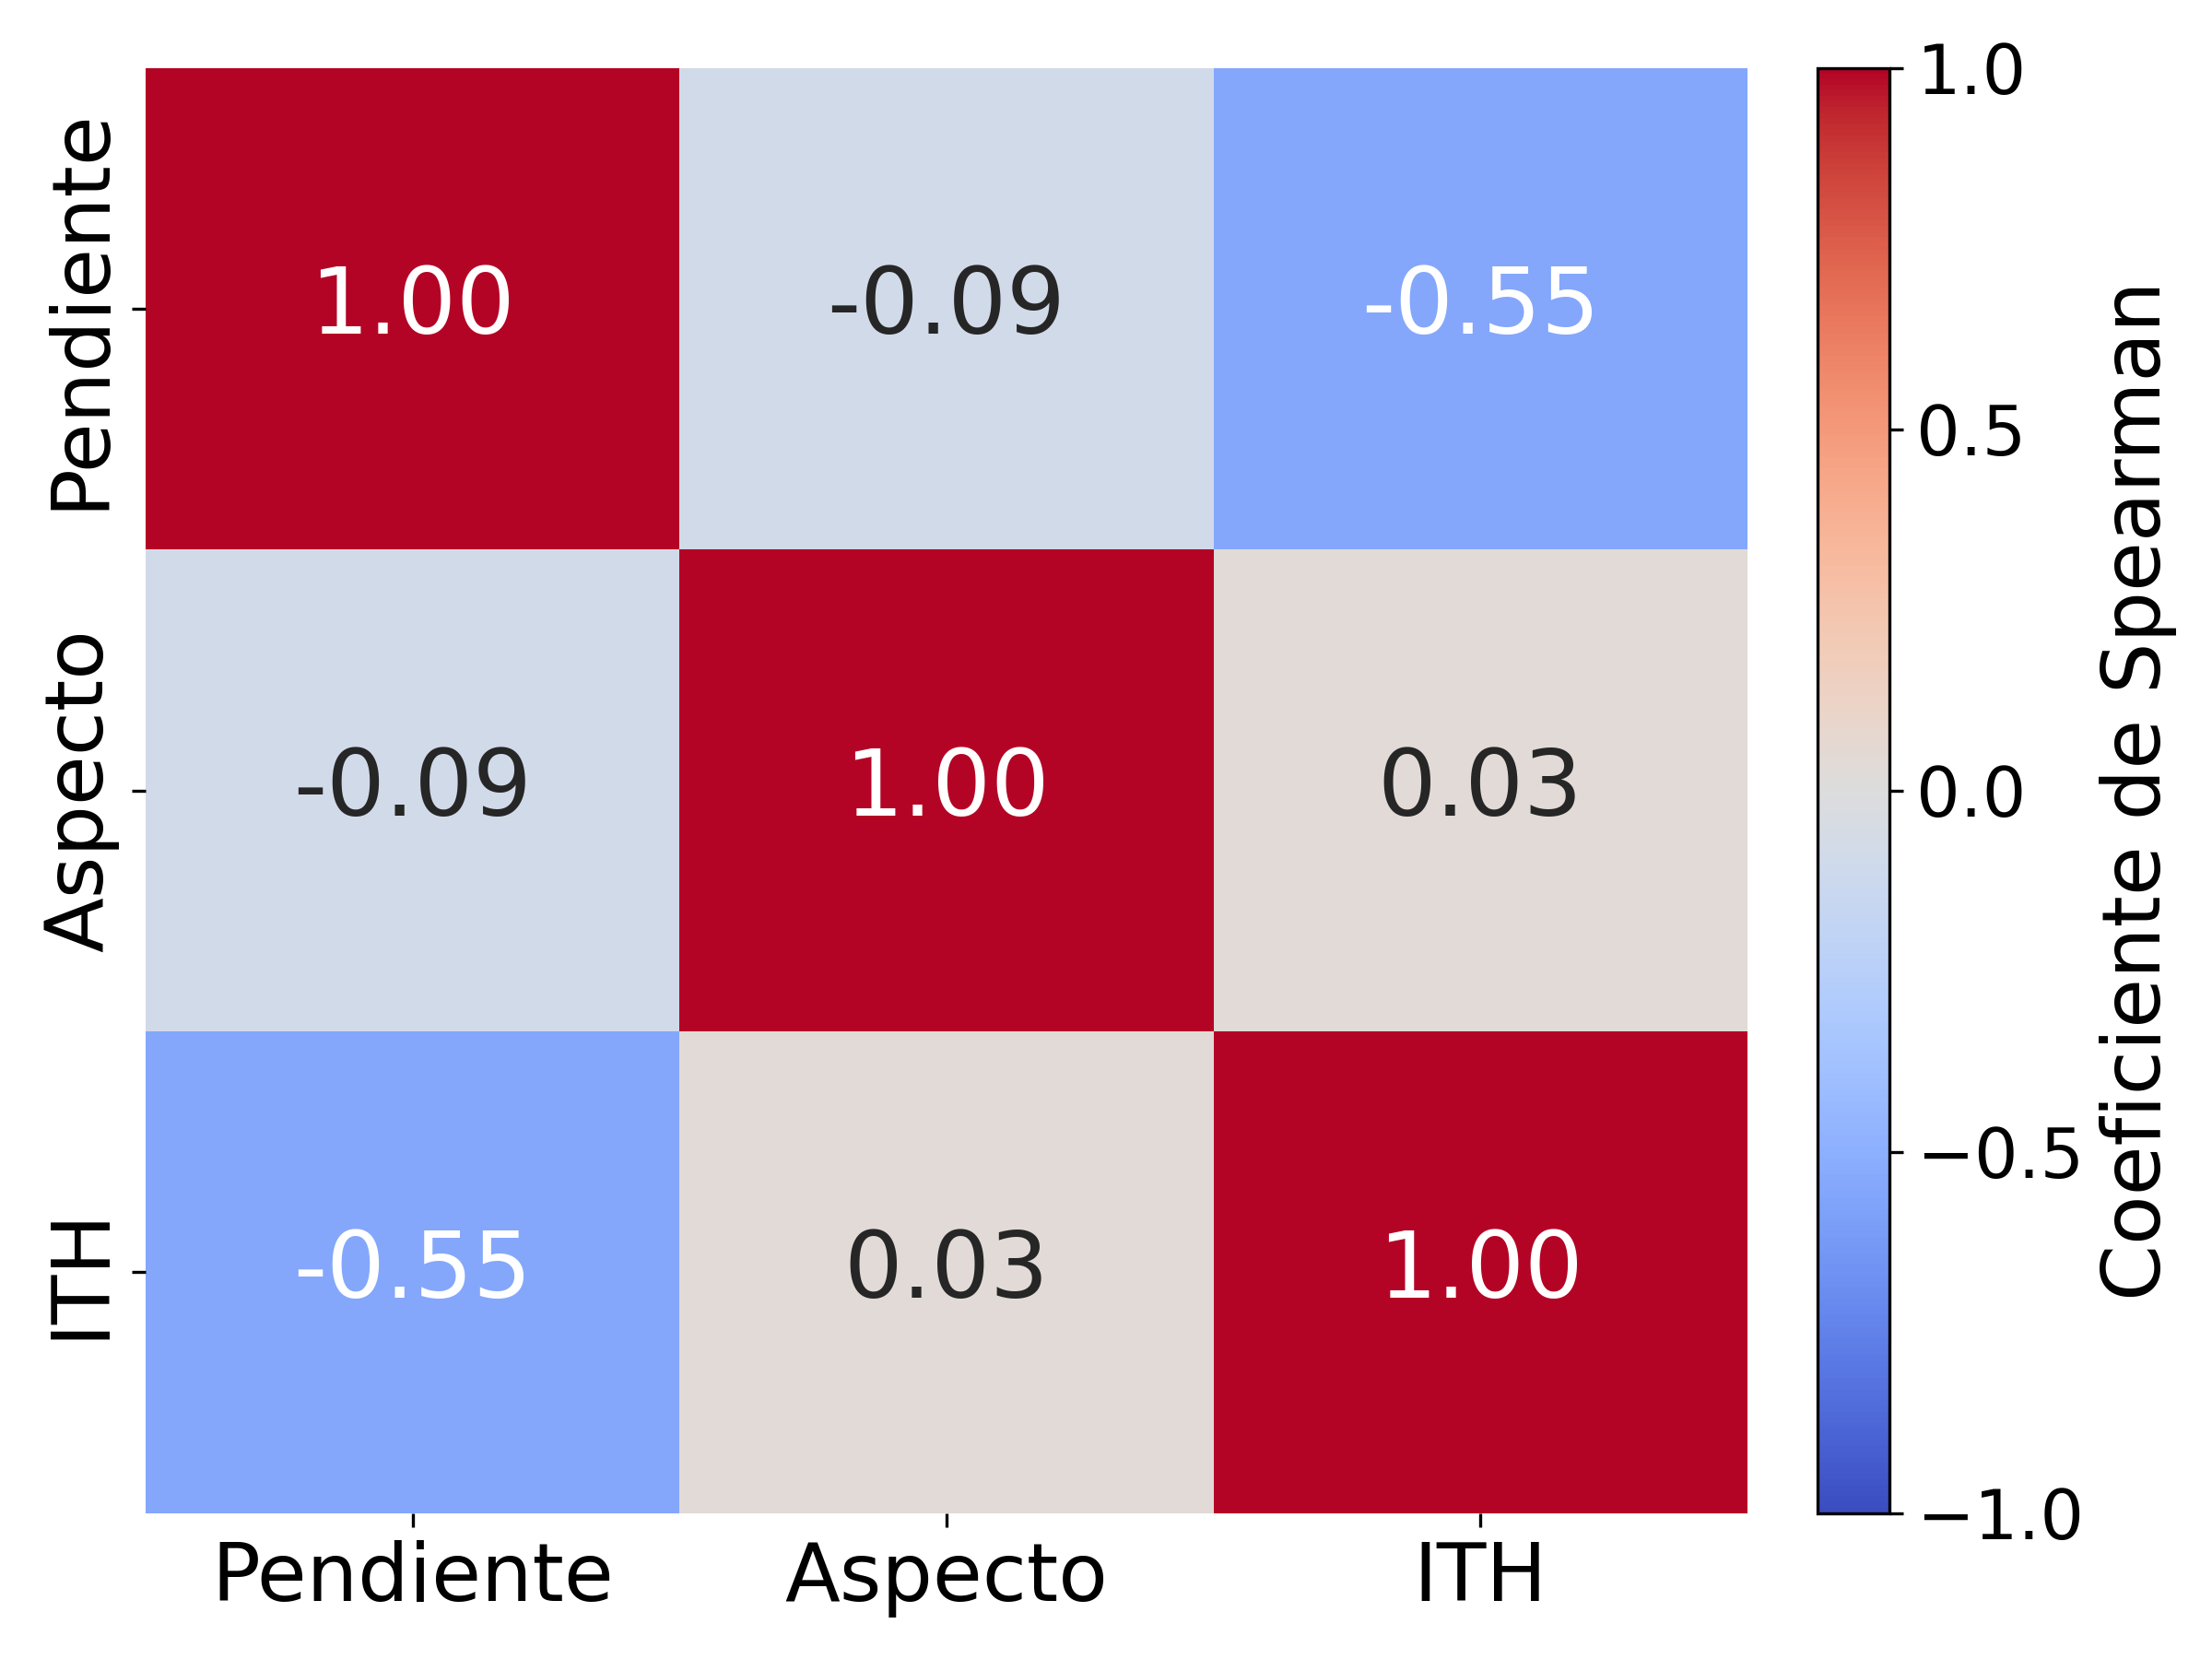
\includegraphics[width=0.60\textwidth]{Fig2_correlation.png}
    \caption{Matriz de correlación de Spearman para las variables topográficas continuas (pendiente, aspecto, ITH).}
    \label{fig:correlacion}
\end{figure}

Las distribuciones de frecuencia (Fig.~\ref{fig:dist_cont}) revelan que los movimientos en masa están sistemáticamente condicionados 
por la pendiente: la distribución en sitios de deslizamiento exhibe una moda desplazada hacia los 35° con sobrerrepresentación 
en el rango 25°--55°. El ITH de los sitios tiende a valores menores que el promedio de la cuenca, reflejando su concentración en 
laderas empinadas; el aspecto no muestra preferencia identificada.

\begin{figure}[H]
    \centering
    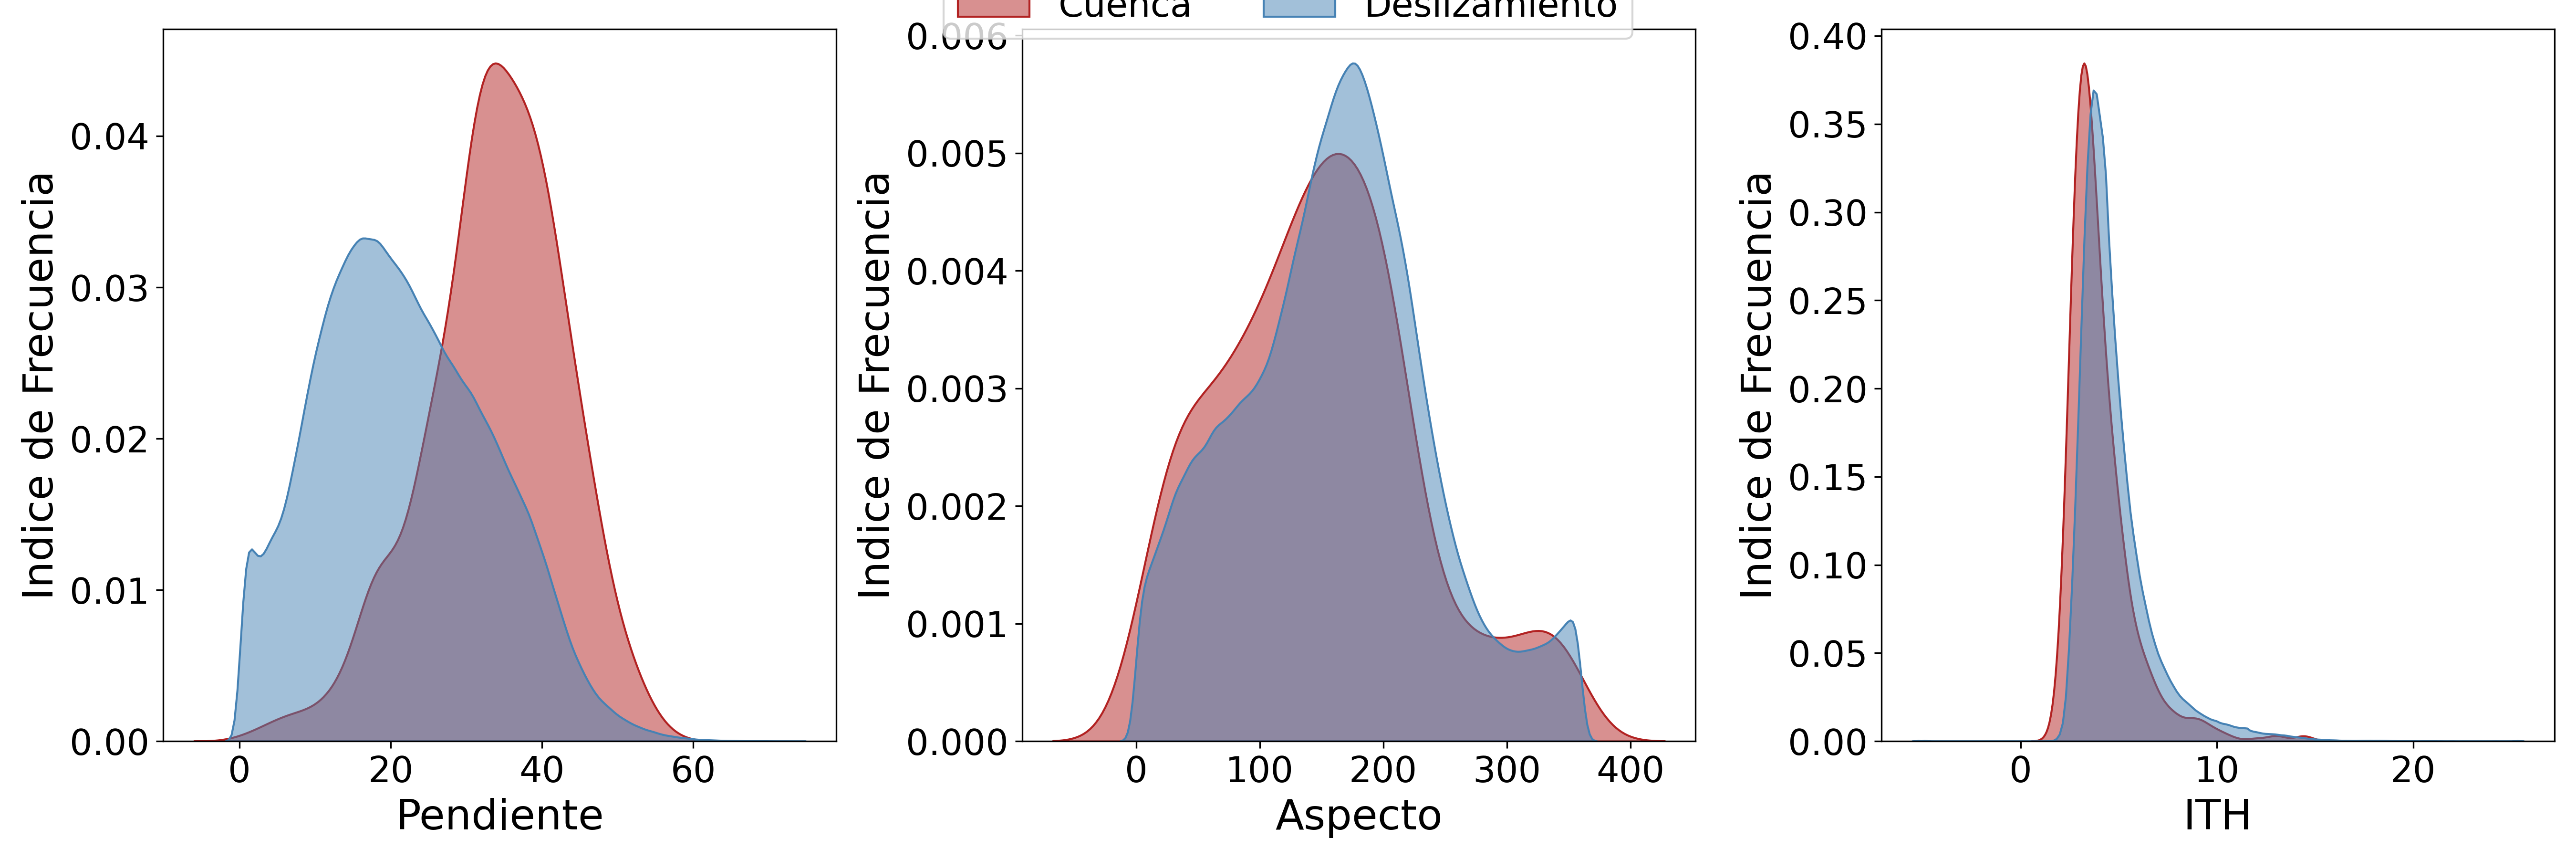
\includegraphics[width=0.9\textwidth]{Fig3_distributions_continuous.png}
    \caption{Distribuciones de densidad de probabilidad empírica (KDE normalizada) para las variables topográficas continuas 
    comparando sitios con deslizamientos (rojo) y la cuenca (azul).}
    \label{fig:dist_cont}
\end{figure}

Las distribuciones categóricas (Fig.~\ref{fig:dist_cat}) muestran que las unidades metamórficas concentran la mayor proporción 
de eventos. Las coberturas de pastos, urbano informal y condominios exhiben un índice de frecuencia relativa superior a su 
representación areal.

\begin{figure}[H]
    \centering
    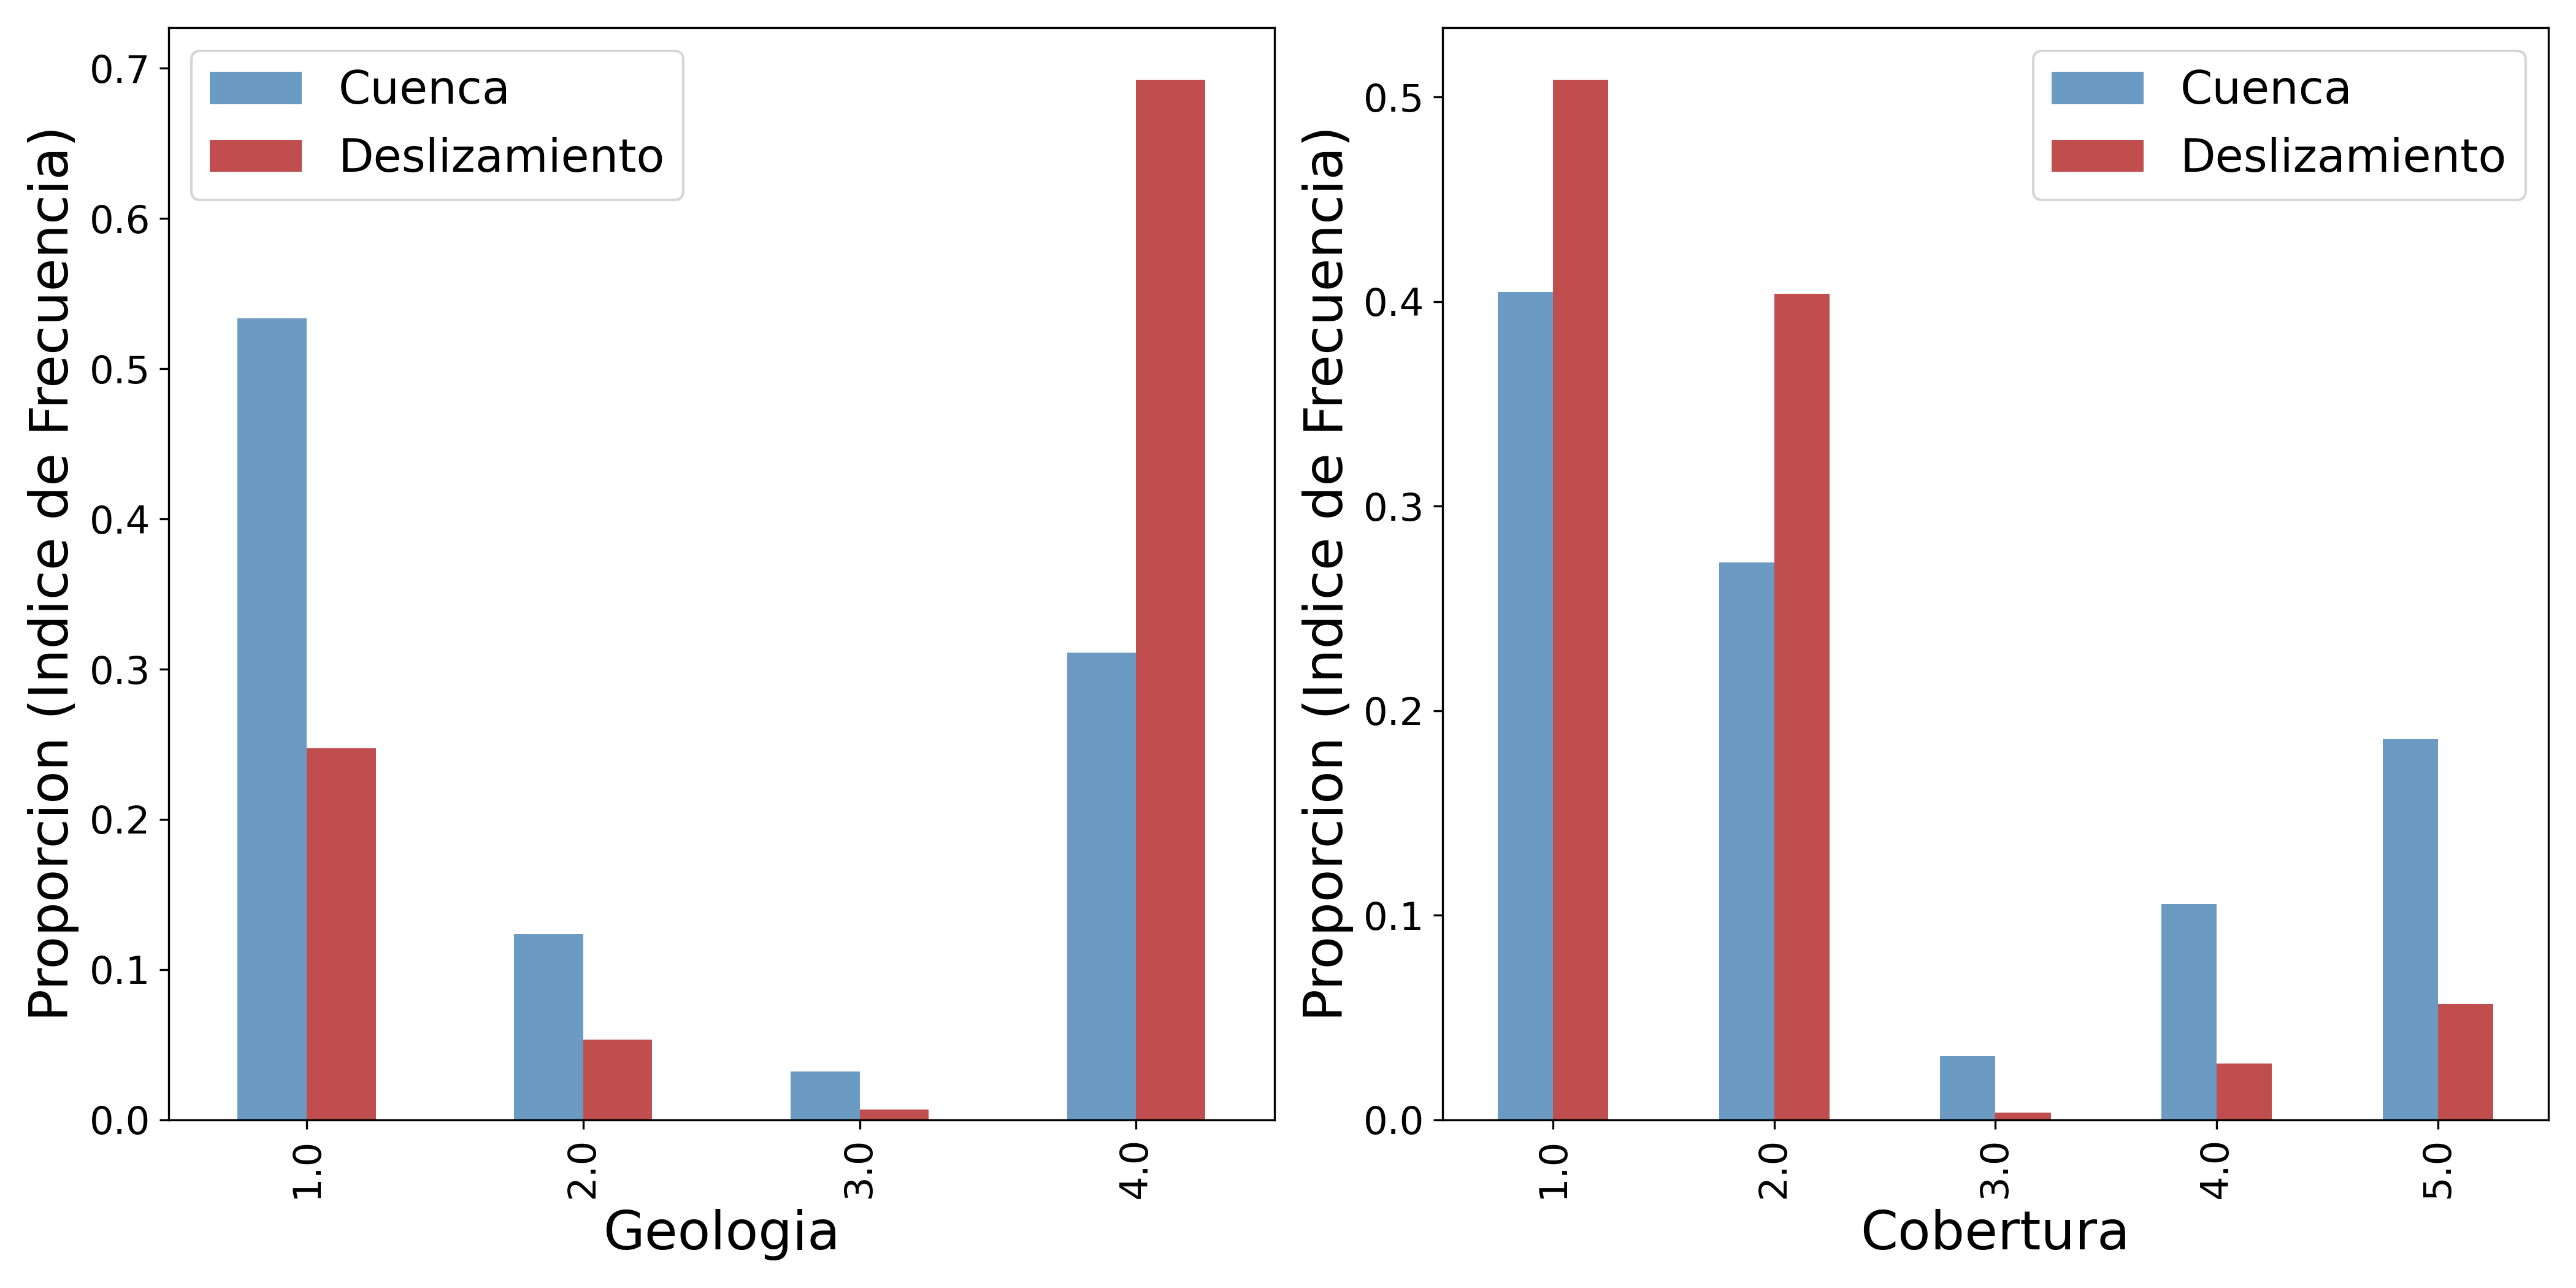
\includegraphics[width=0.9\textwidth]{Fig4_distributions_categorical.png}
    \caption{Índice de frecuencia proporcional para las variables categóricas. Barras azules: proporción de área de cada clase; 
    barras rojas: proporción de deslizamientos.}
    \label{fig:dist_cat}
\end{figure}

La Fig.~\ref{fig:kde_map} muestra la superficie de densidad KDE normalizada del inventario ($h \approx 691$~m). Los núcleos de 
máxima densidad se concentran en las laderas medias de los tributarios noroccidentales, donde la coexistencia de pendientes 
fuertes sobre rocas metamórficas y cobertura de pastos o urbano informal genera las condiciones de mayor ocurrencia de deslizamientos. 
Esta superficie constituye la variable de respuesta del primer enfoque de modelado (PGR).

\begin{figure}[H]
    \centering
    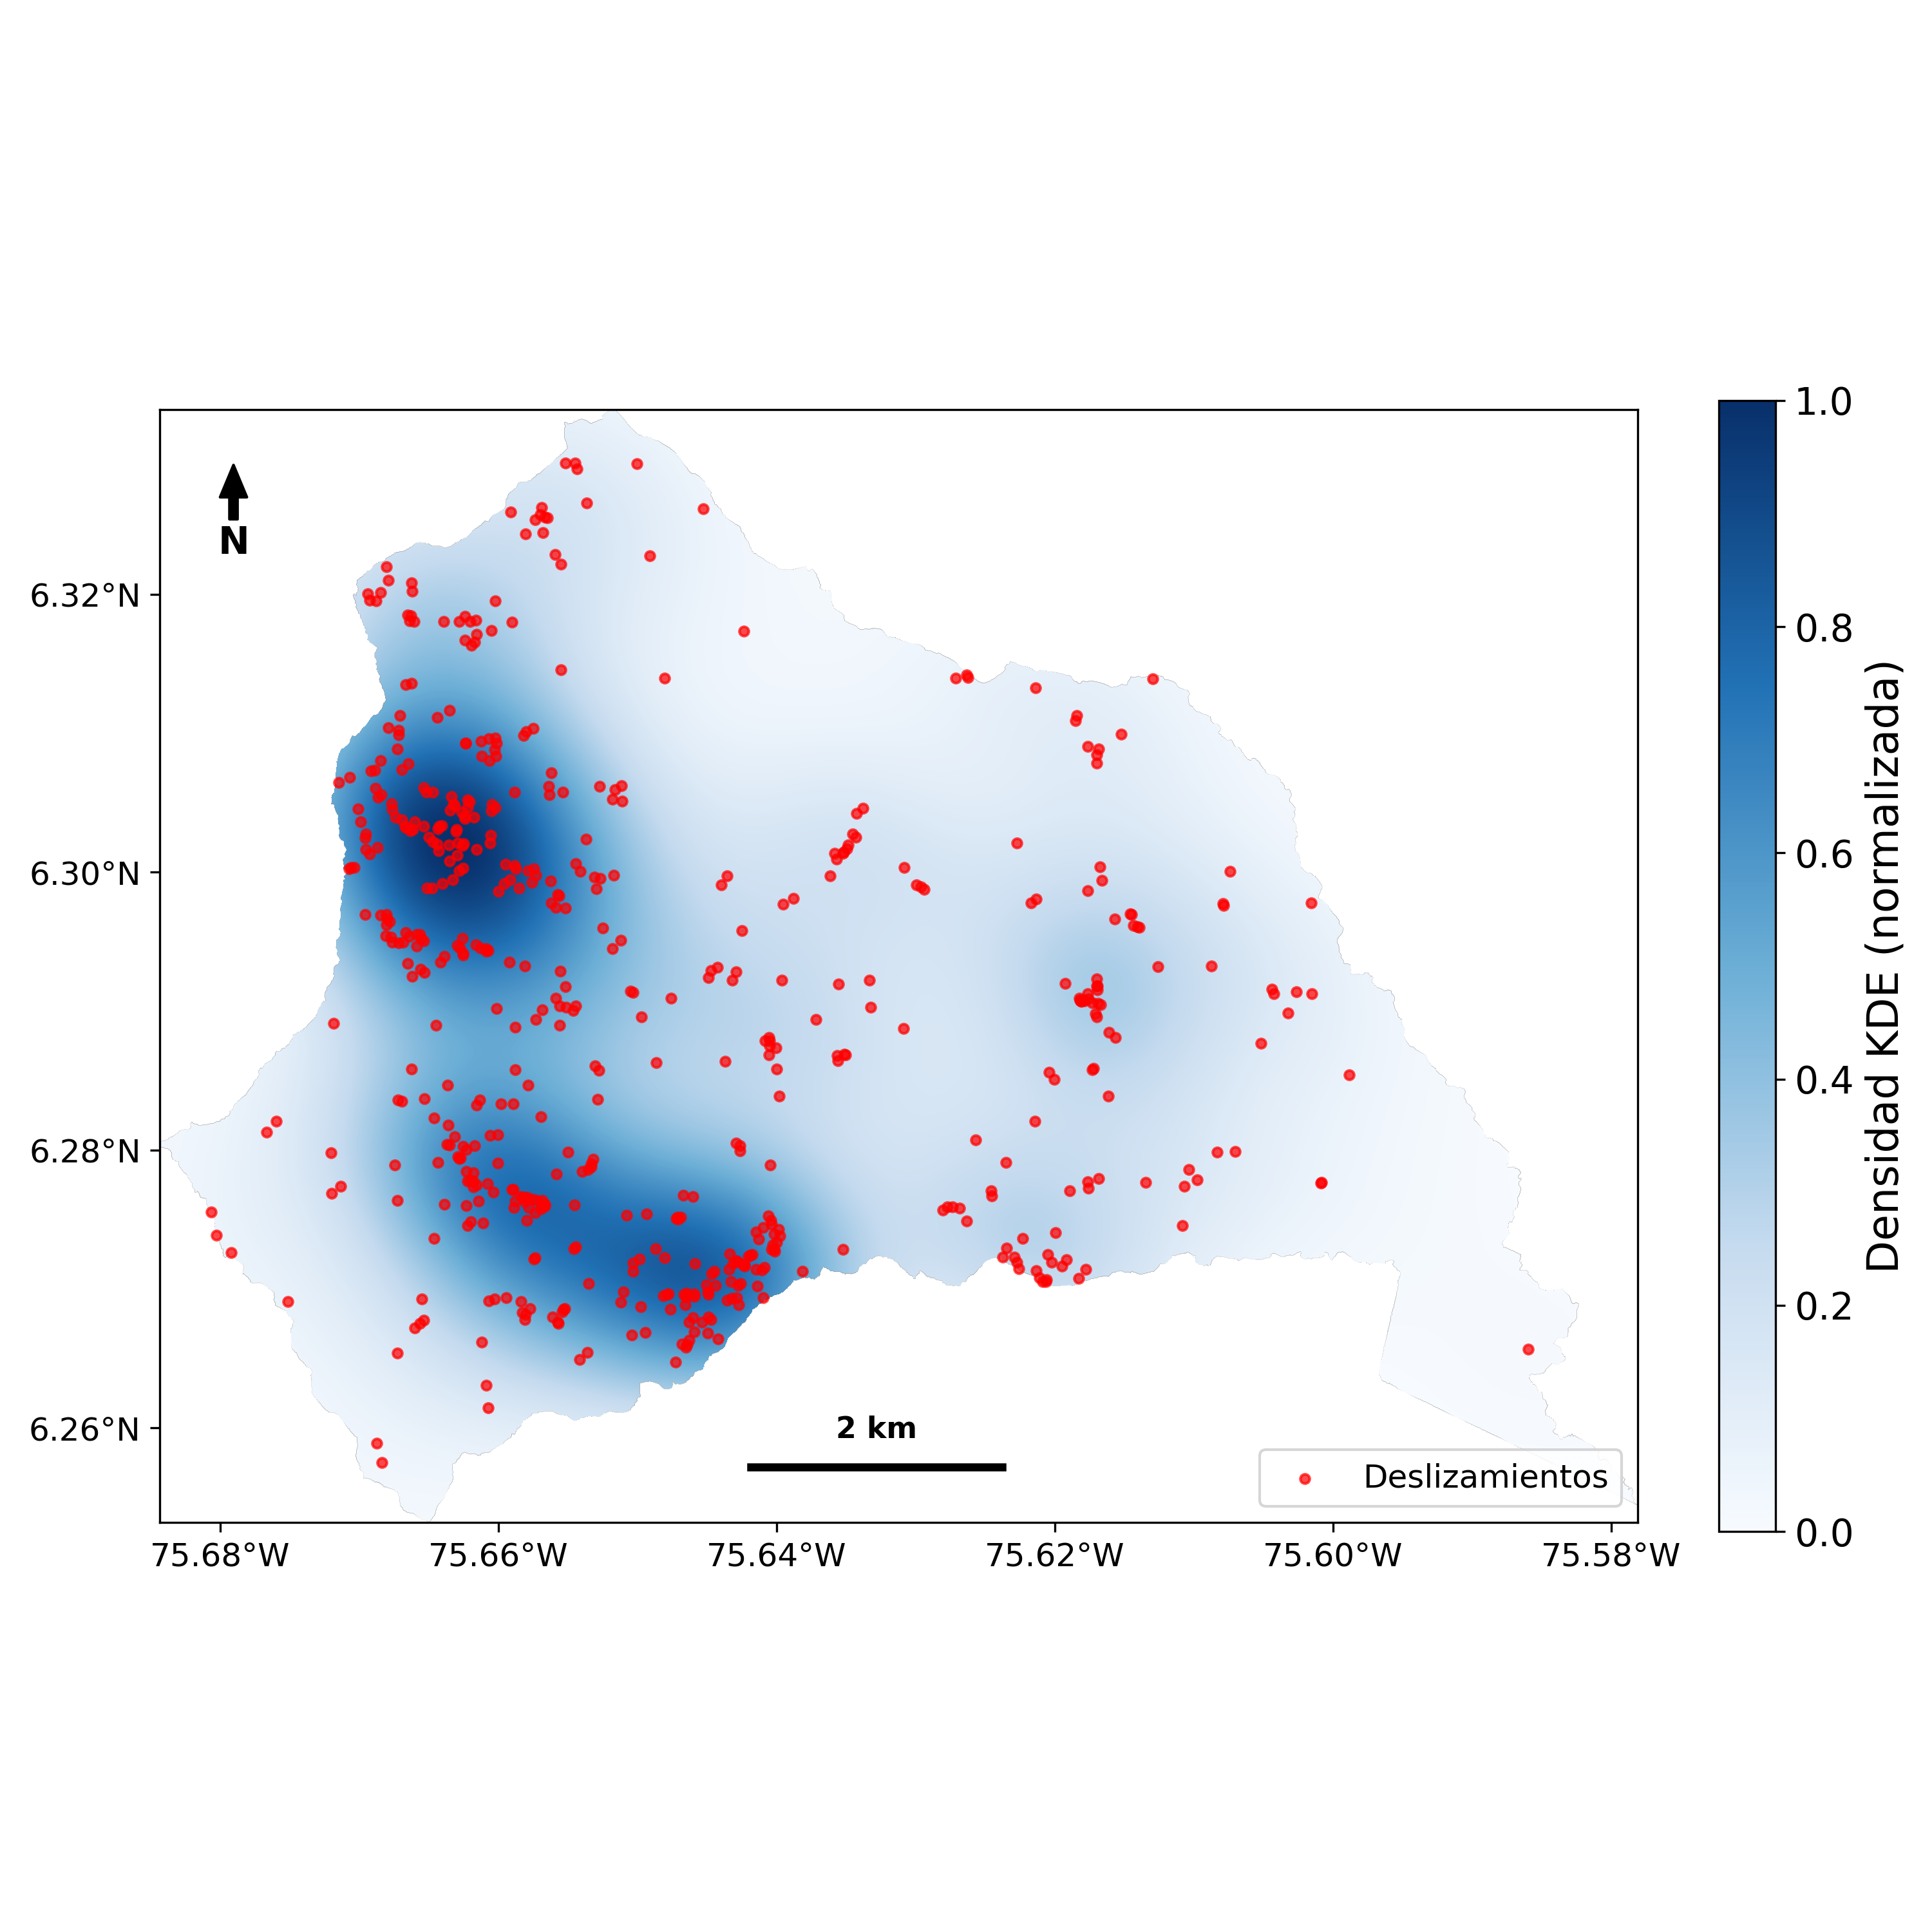
\includegraphics[width=0.85\textwidth]{Fig5_kde_map.png}
    \caption{Mapa de densidad KDE (normalizada, $[0,1]$) del inventario de 583 deslizamientos (puntos rojos). El ancho de banda 
    de Silverman ($h \approx 691$~m) captura los núcleos de agregación espacial de eventos en las laderas medias noroccidentales 
    de la cuenca.}
    \label{fig:kde_map}
\end{figure}

La Tabla~\ref{tab:pgr_kde} y la Fig.~\ref{fig:roc_pgr} presentan los resultados del PGR para los 
modelos univariados y multivariados. Los modelos univariados revelan que las variables categóricas son las más informativas para
predecir la densidad KDE del inventario. La geología sola alcanza el mayor AUC (0{,}694), seguida de la cobertura del suelo
(0{,}631); las variables topográficas continuas (pendiente, aspecto, ITH) se sitúan apenas por encima del nivel aleatorio
(AUC~$\approx$~0{,}550). Considerando que el aspecto no señaló un patrón diferencial entre celdas con y sin deslizamientos 
y que ITH se correlaciona inversamente con la pendiente,
se utilizo un modelo de tres variables (pendiente~+~geología~+~cobertura) que obtiene AUC~=~0{,}559, por debajo de la geología sola, 
evidenciando que la combinación de covariables no beneficia sustancialmente al PGR.
El modelo con las cinco variables alcanza AUC~=~0{,}698, el mayor de todos. La correlación de Pearson
entre las predicciones del PGR de tres variables y la superficie KDE objetivo fue $r = 0{,}061$ (RMSE~=~0{,}255), confirmando
que ninguna configuración logra reproducir adecuadamente la superficie de densidad. El mapa de susceptibilidad derivado del PGR
 (Fig.~\ref{fig:gpr_susc}) muestra una distribución espacialmente difusa sin la coherencia geomorfológica esperada.

 \begin{table}[H]
    \centering
    \caption{Resultados del PGR para modelos univariados y multivariados. AUC: área bajo la curva ROC; AP: precisión media; Brier: puntuación de Brier.}
    \label{tab:pgr_kde}
    \begin{tabular}{lcccc}
        \toprule
        Modelo PGR & $N$ var. & AUC-ROC & AP & Brier \\
        \midrule
        \quad Geología & 1 & 0{,}694 & 0{,}001 & 0{,}335 \\
        \quad Cobertura del suelo & 1 & 0{,}631 & 0{,}000 & 0{,}571 \\
        \quad ITH & 1 & 0{,}550 & 0{,}015 & 0{,}151 \\
        \quad Aspecto & 1 & 0{,}550 & 0{,}041 & 0{,}151 \\
        \quad Pendiente & 1 & 0{,}543 & 0{,}048 & 0{,}150 \\
        \quad Pendiente + Geología + Cobertura & 3 & 0{,}559 & 0{,}017 & 0{,}151 \\
        \quad todas las variables & 5 & 0{,}698 & 0{,}002 & 0{,}130 \\
        \bottomrule
    \end{tabular}
\end{table}

\begin{figure}[H]
    \centering
    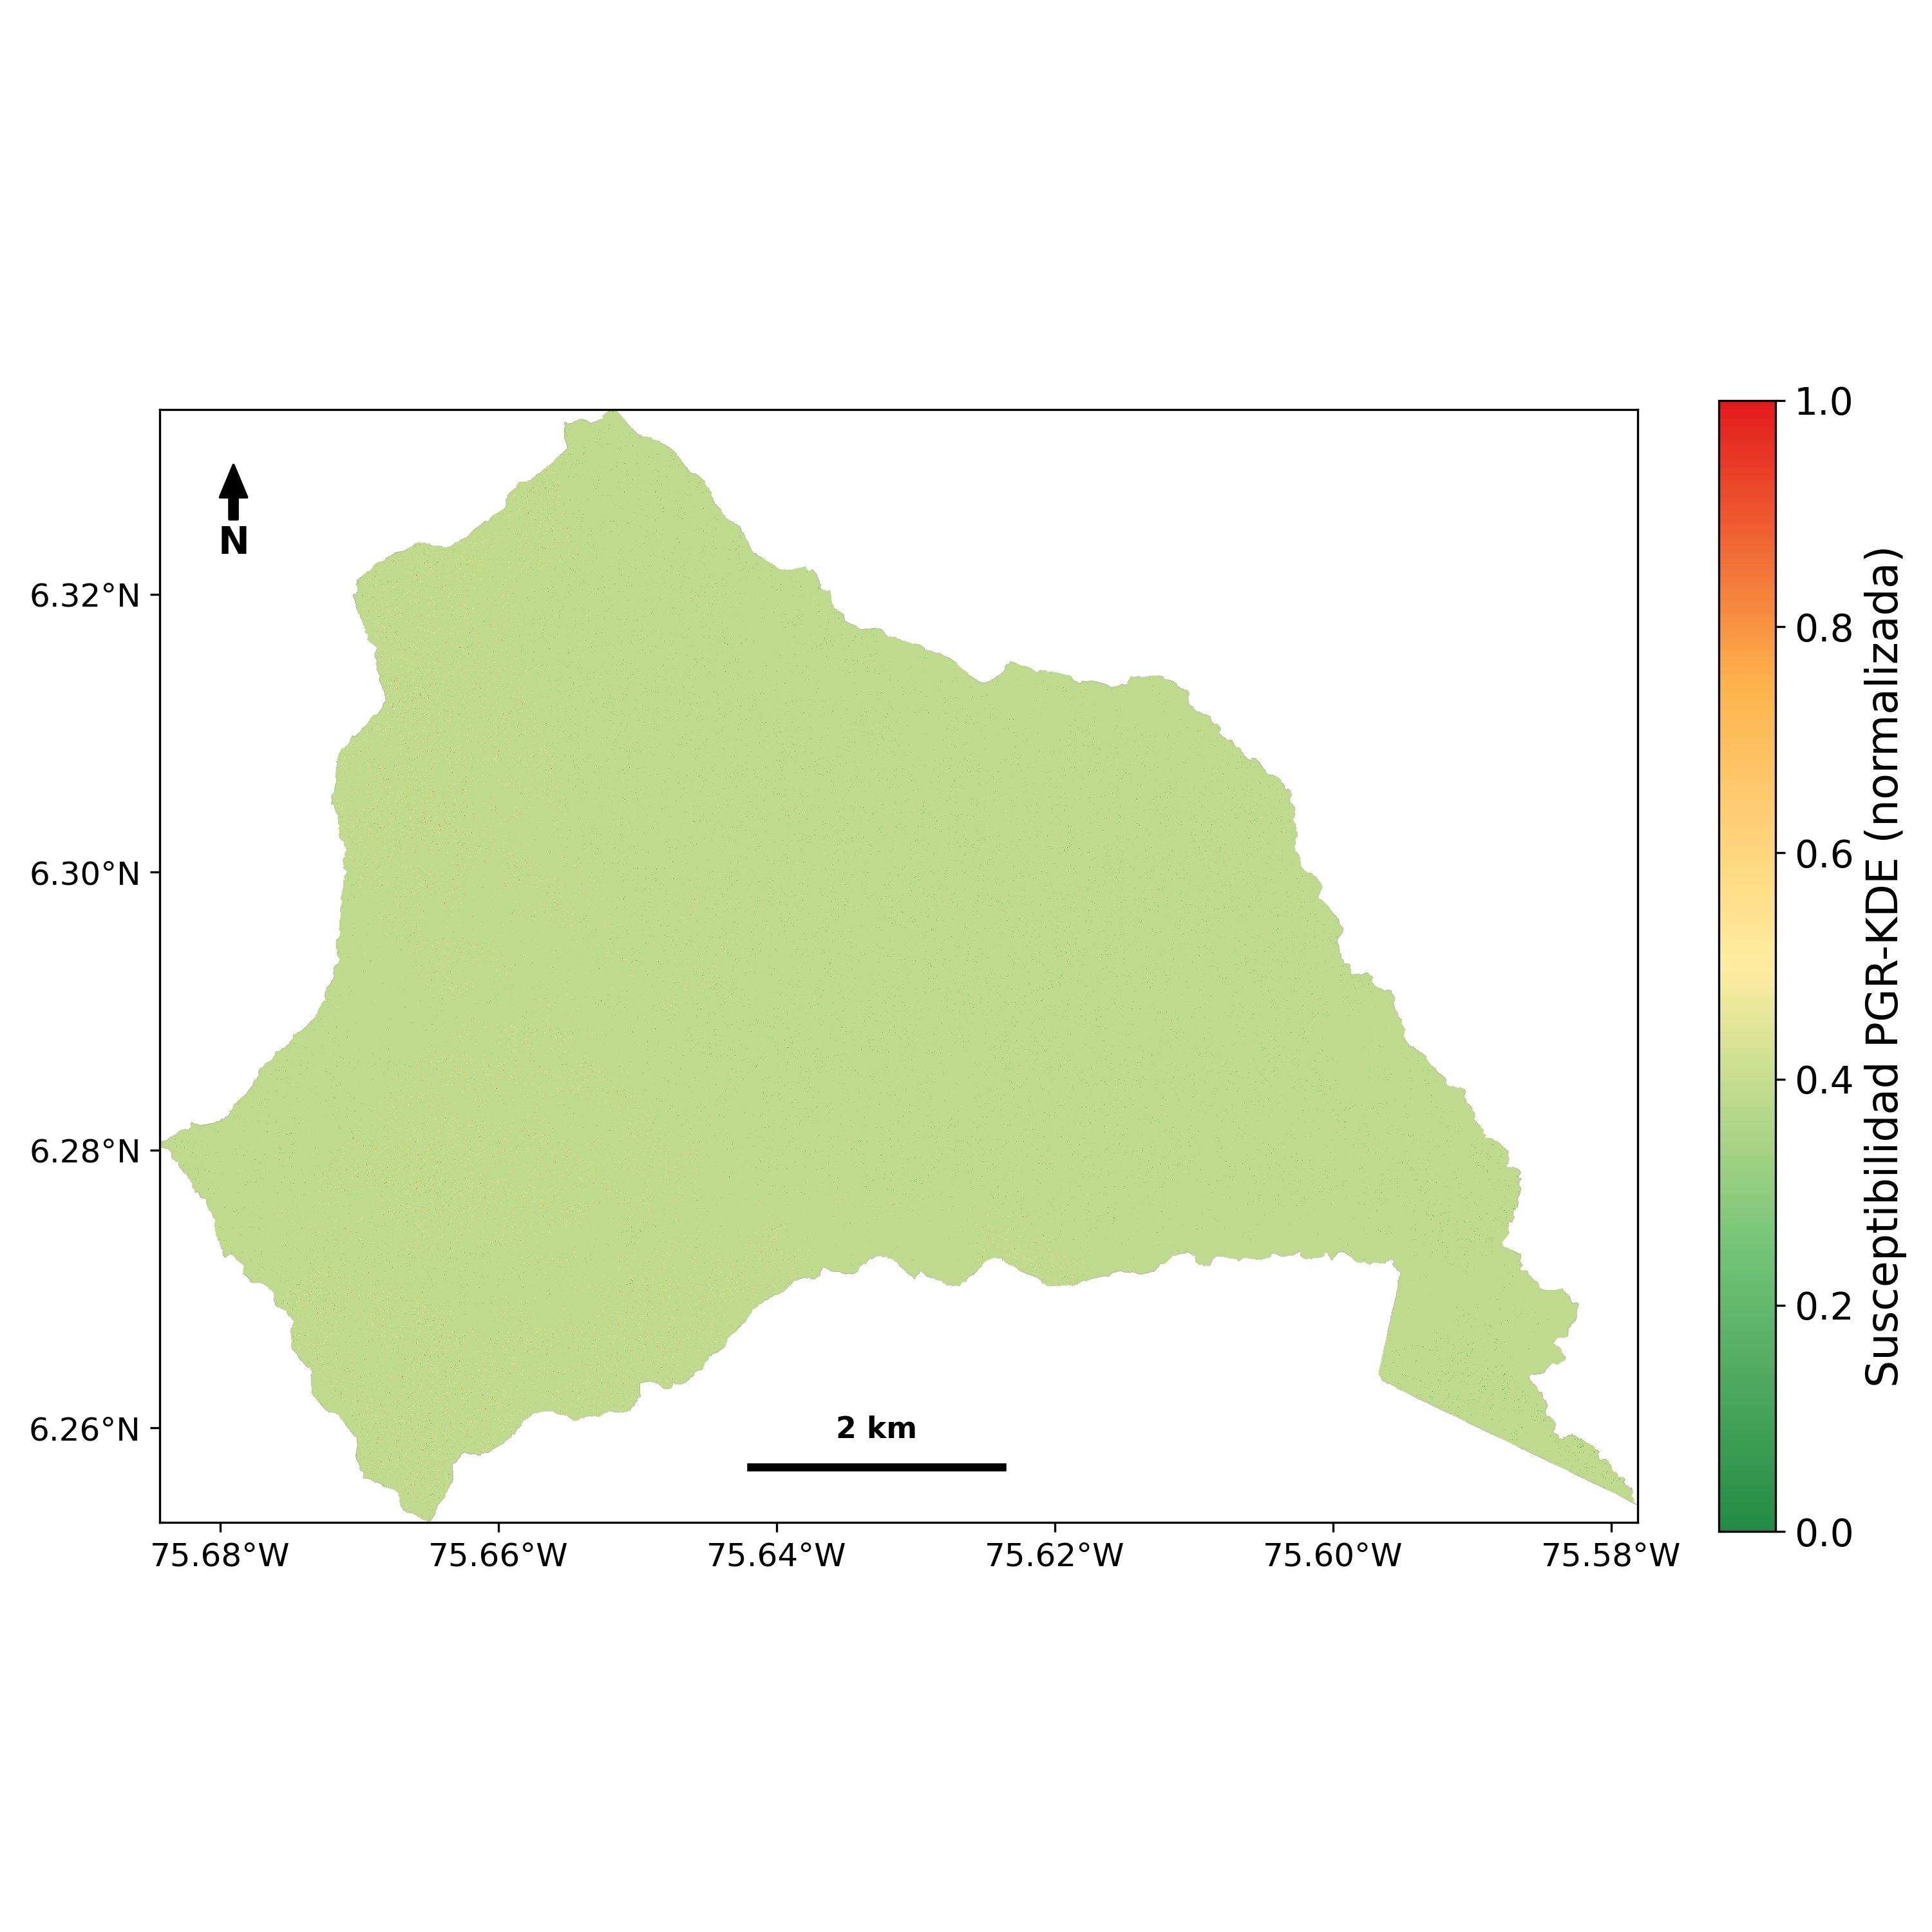
\includegraphics[width=0.85\textwidth]{Fig7_gpr_susceptibility.png}
    \caption{Mapa de susceptibilidad derivado del PGR (predicción normalizada a $[0,1]$). El modelo PGR
    no logra reproducir la superficie KDE con las covariables locales (AUC~=~0{,}559).}
    \label{fig:gpr_susc}
\end{figure}

\begin{figure}[H]
    \centering
    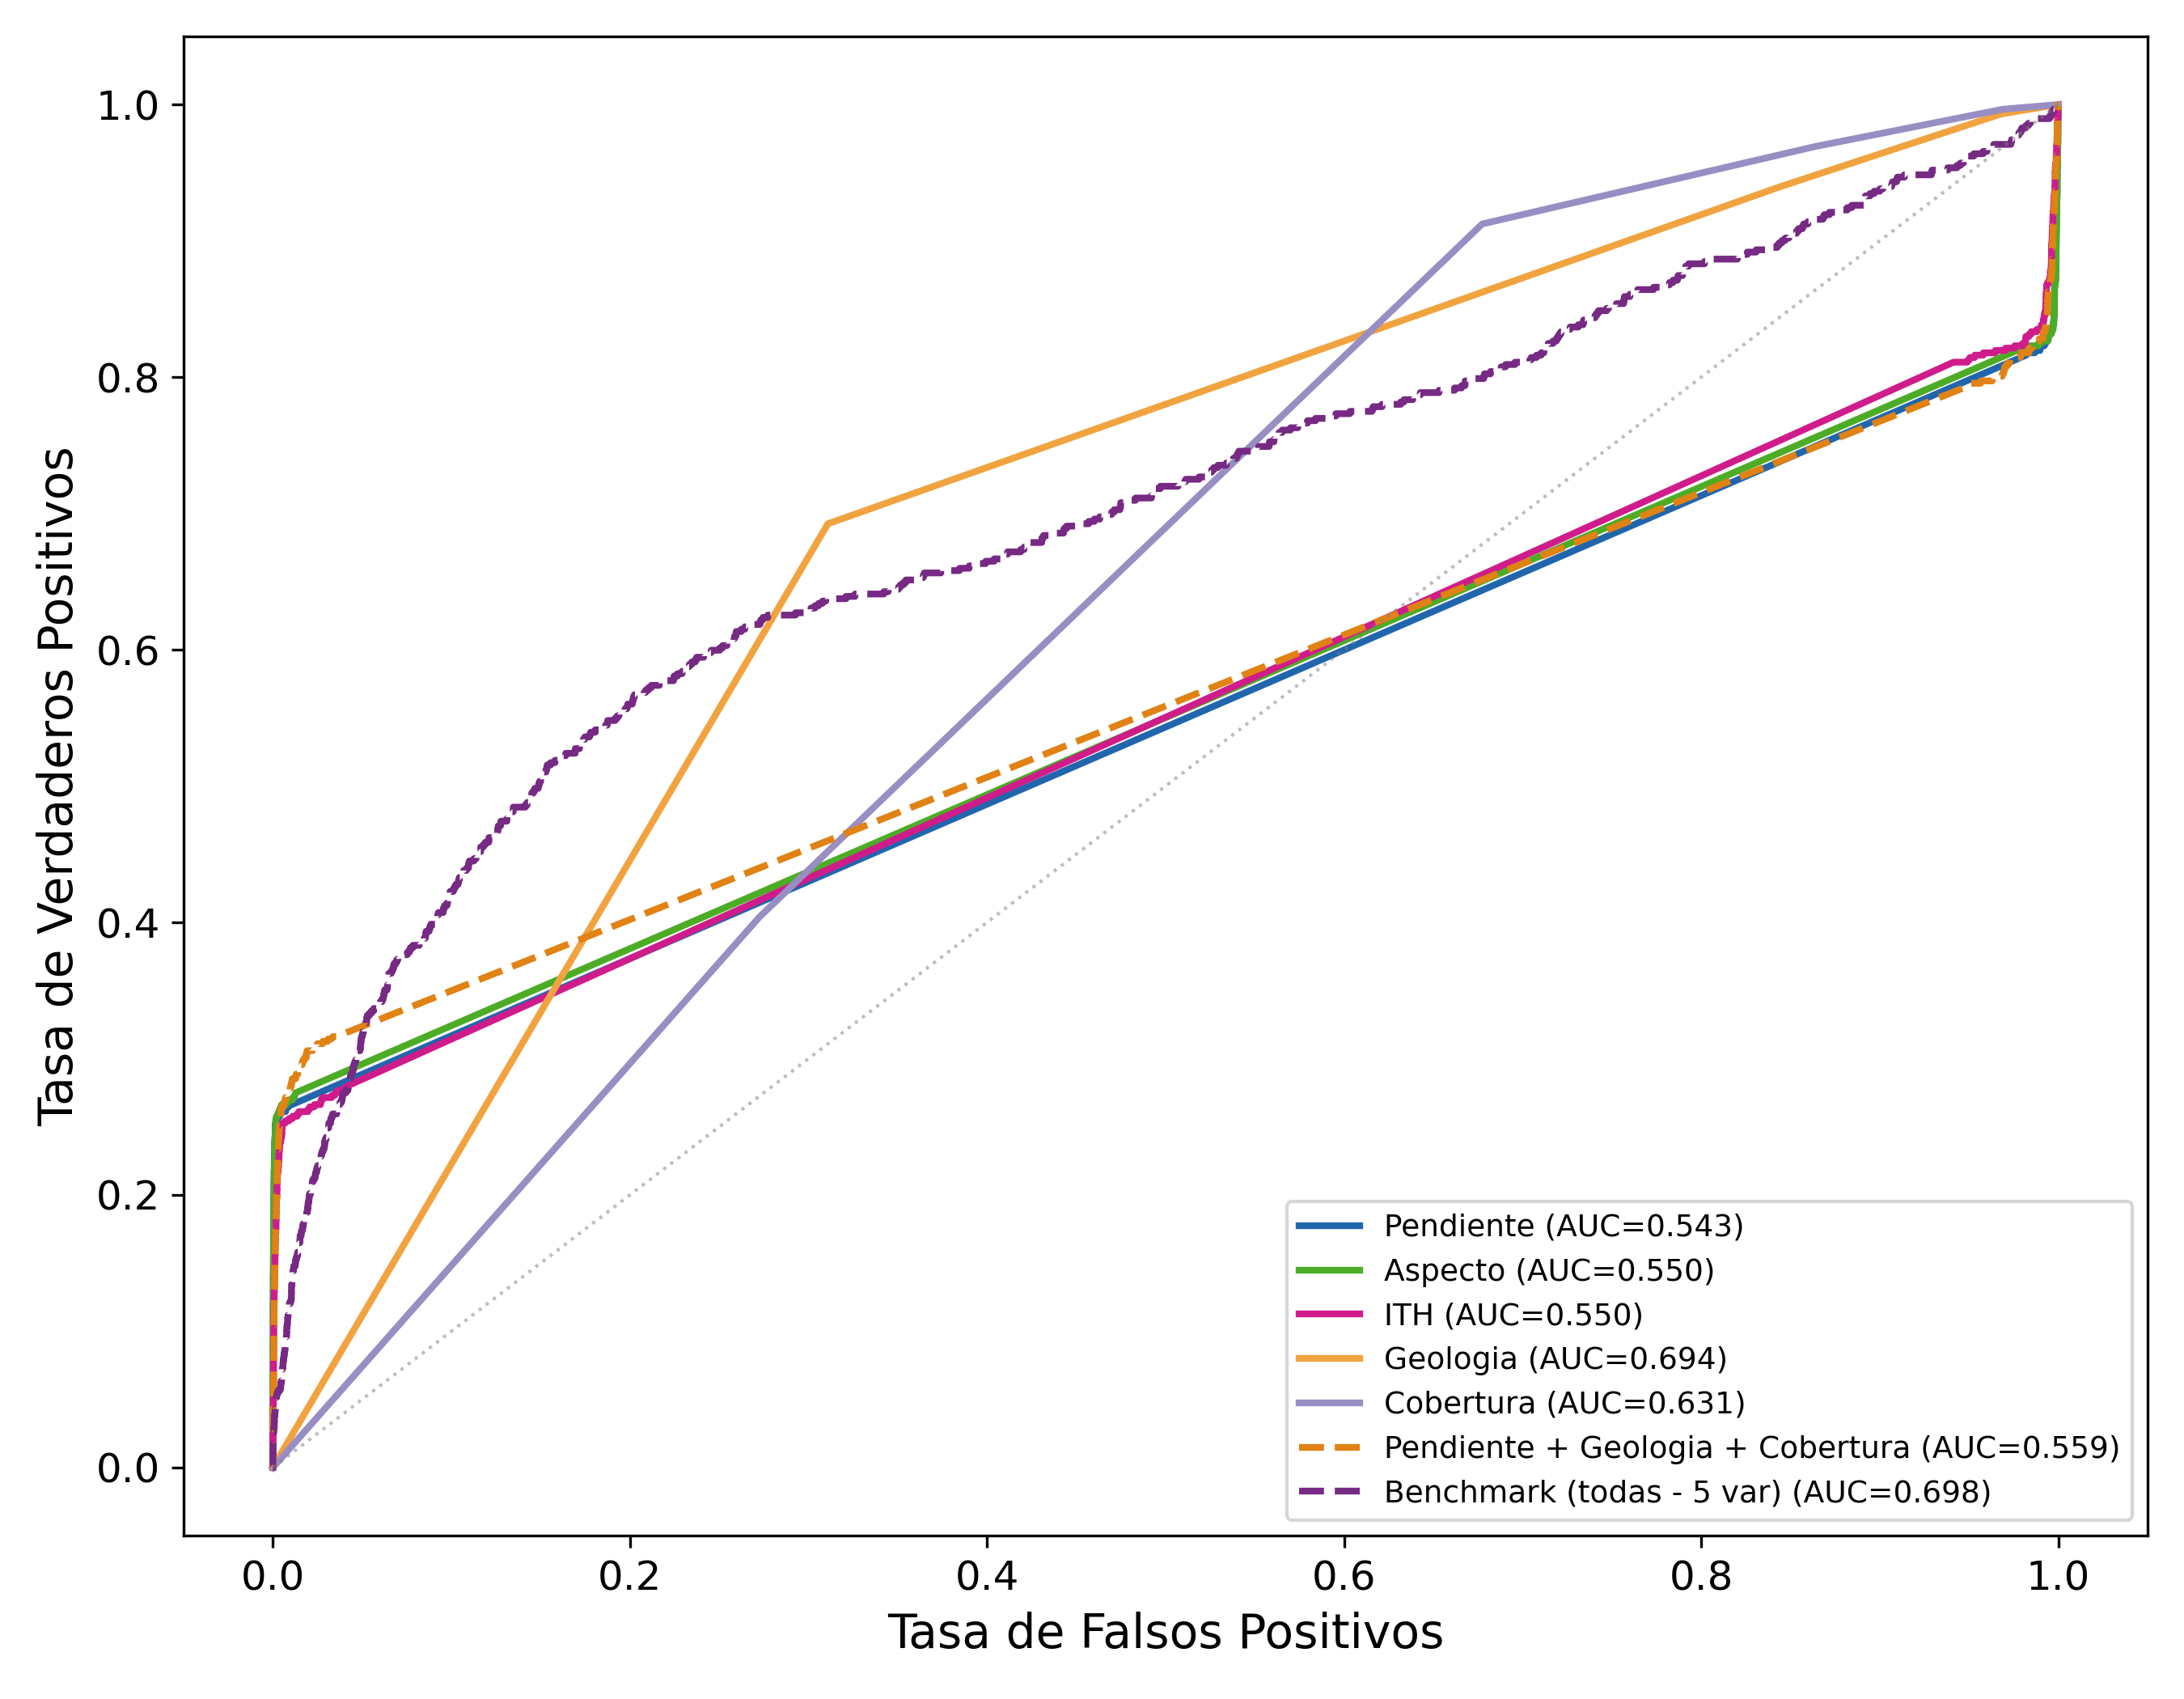
\includegraphics[width=0.72\textwidth]{Fig6_roc_pgr_kde.png}
    \caption{Curvas ROC para todas las configuraciones del PGR: cinco modelos univariados y dos
    modelos multivariados (pendiente~+~geología~+~cobertura y \textit{toas las variables}). 
    Las curvas se agrupan ligeramente por encima de un modelo aleatorio (AUC entre 0{,}543 y 0{,}698).}
    \label{fig:roc_pgr}
\end{figure}

El mapa de incertidumbre del PGR (Fig.~\ref{fig:pgr_std}) exhibe el patrón complementario esperado: la desviación estándar posterior
más elevada aparece en los extremos de la cuenca, que representan combinaciones de covariables escasamente representadas en el
inventario. Las laderas medias, donde la densidad del inventario es mayor, presentan menor incertidumbre.

\begin{figure}[H]
    \centering
    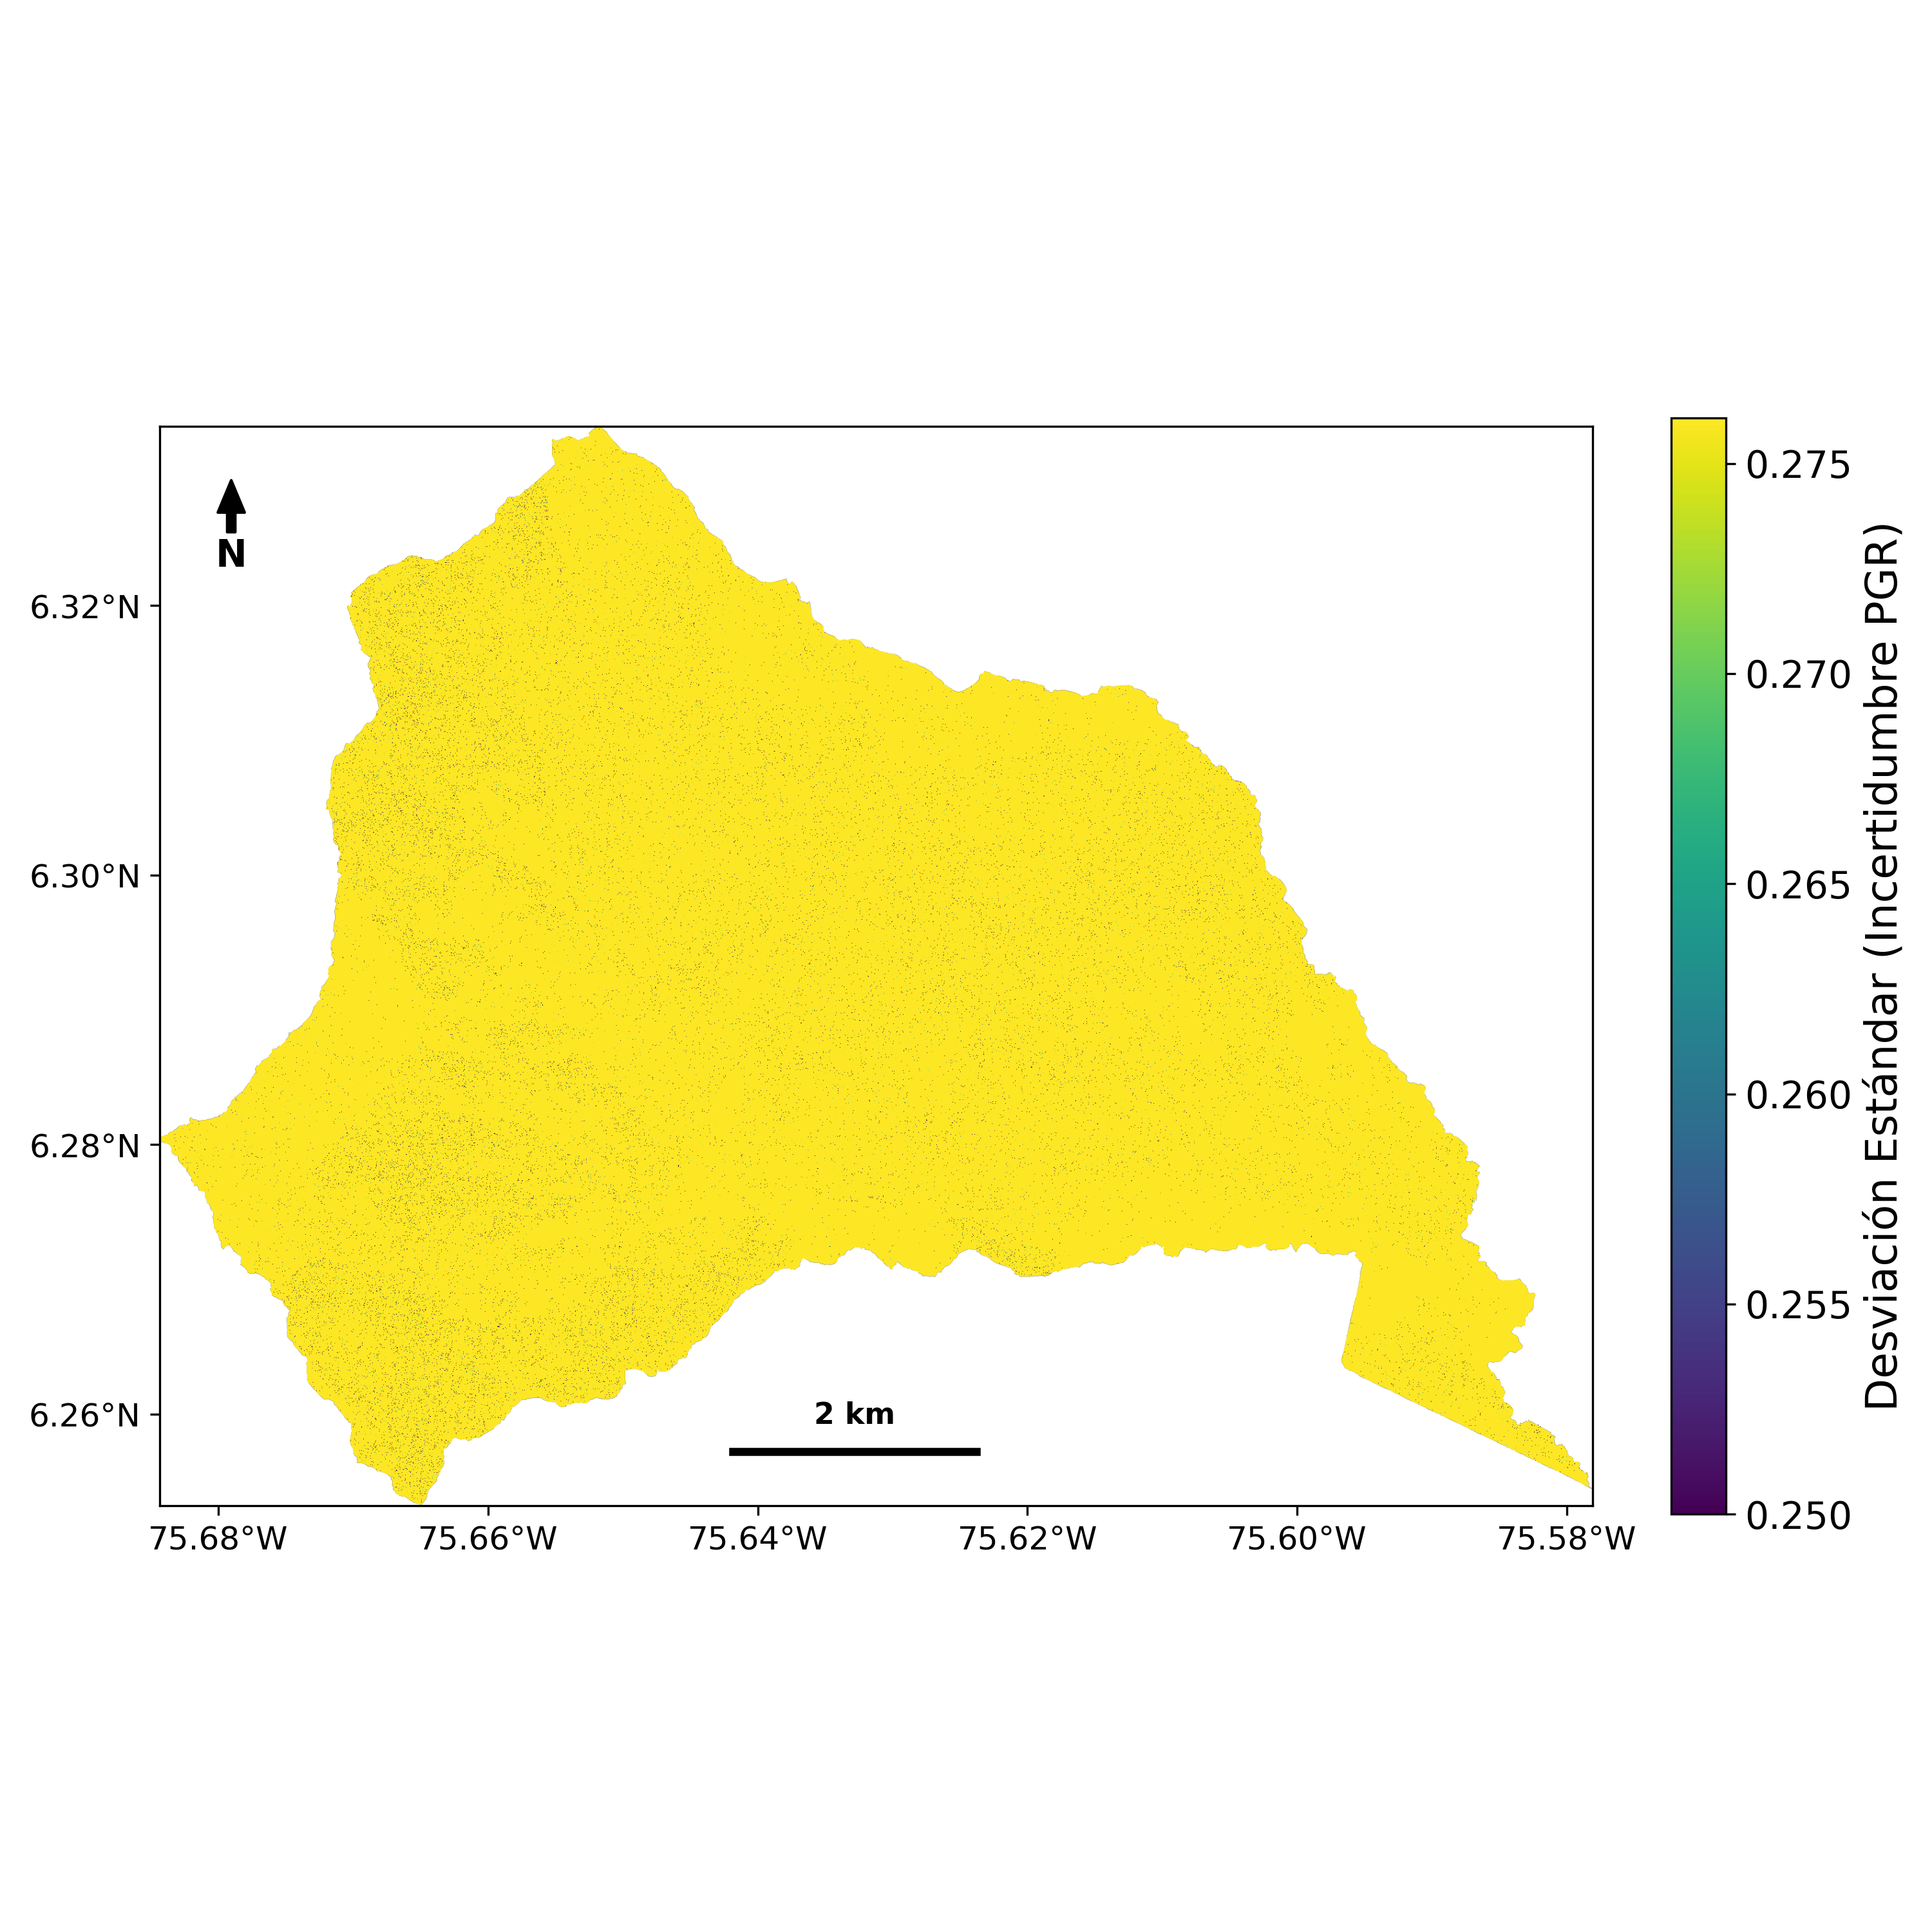
\includegraphics[width=0.85\textwidth]{Fig_pgr_std.png}
    \caption{Mapa de incertidumbre espacial (desviación estándar posterior) del PGR. Valores altos indican zonas donde la predicción 
    del PGR está pobremente restringida por los datos históricos; se concentran en los extremos de la cuenca, escasamente 
    cubiertos por el inventario.}
    \label{fig:pgr_std}
\end{figure}

La Fig.~\ref{fig:roc_pgc} y la Tabla~\ref{tab:pgc} presentan las curvas ROC y los valores de AUC 
para las configuraciones del PGC. Dentro del PGC, el modelo con todas las variables alcanzó el AUC más alto (0{,}826). 
El modelo topográfico puro (0{,}793) supera al categórico puro (0{,}742), confirmando que la topografía es el predictor 
estructuralmente más potente en conjunto. El modelo de tres variables (pendiente, geología y cobertura) alcanza AUC~=~0{,}823, 
prácticamente idéntico al \textit{todas las variables} (0{,}826), señalando que el aspecto y el ITH son redundantes cuando la geología y 
la cobertura ya están incluidas.

\begin{table}[H]
    \centering
    \caption{Resultados de las cuatro configuraciones del PGC evaluadas sobre la cuenca. Los valores en
    negrita indican los modelos seleccionados por su desempeño. AUC: área bajo la curva ROC; AP: precisión media; Brier:
    puntuación de Brier.}
    \label{tab:pgc}
    \begin{tabular}{lcccc}
        \toprule
        Modelo PGC & $N$ var. & AUC-ROC & AP & Brier \\
        \midrule
        \textbf{(todas las variables)} & 5 & \textbf{0{,}826} & 0{,}001 & 0{,}188 \\
        \textbf{Pendiente + Geología + Cobertura} & 3 & \textbf{0{,}823} & 0{,}002 & 0{,}190 \\
        Solo topografía & 3 & 0{,}793 & 0{,}001 & 0{,}195 \\
        Solo geoespacial & 2 & 0{,}742 & 0{,}001 & 0{,}220 \\
        \bottomrule
    \end{tabular}
\end{table}

El mapa del modelo PGC con mejor desempeño (Fig.~\ref{fig:mapa_final}) muestra una zonificación coherente con la geomorfología: los valores más 
altos (susceptibilidad~$> 0{,}6$) se concentran en las laderas medias sobre suelos derivados de rocas metamórficas con pendientes fuertes, 
particularmente en los tributarios orientados al norte y noroccidente; el fondo del valle y los filos de divisoria exhiben 
valores bajos ($< 0{,}3$).

\begin{figure}[H]
    \centering
    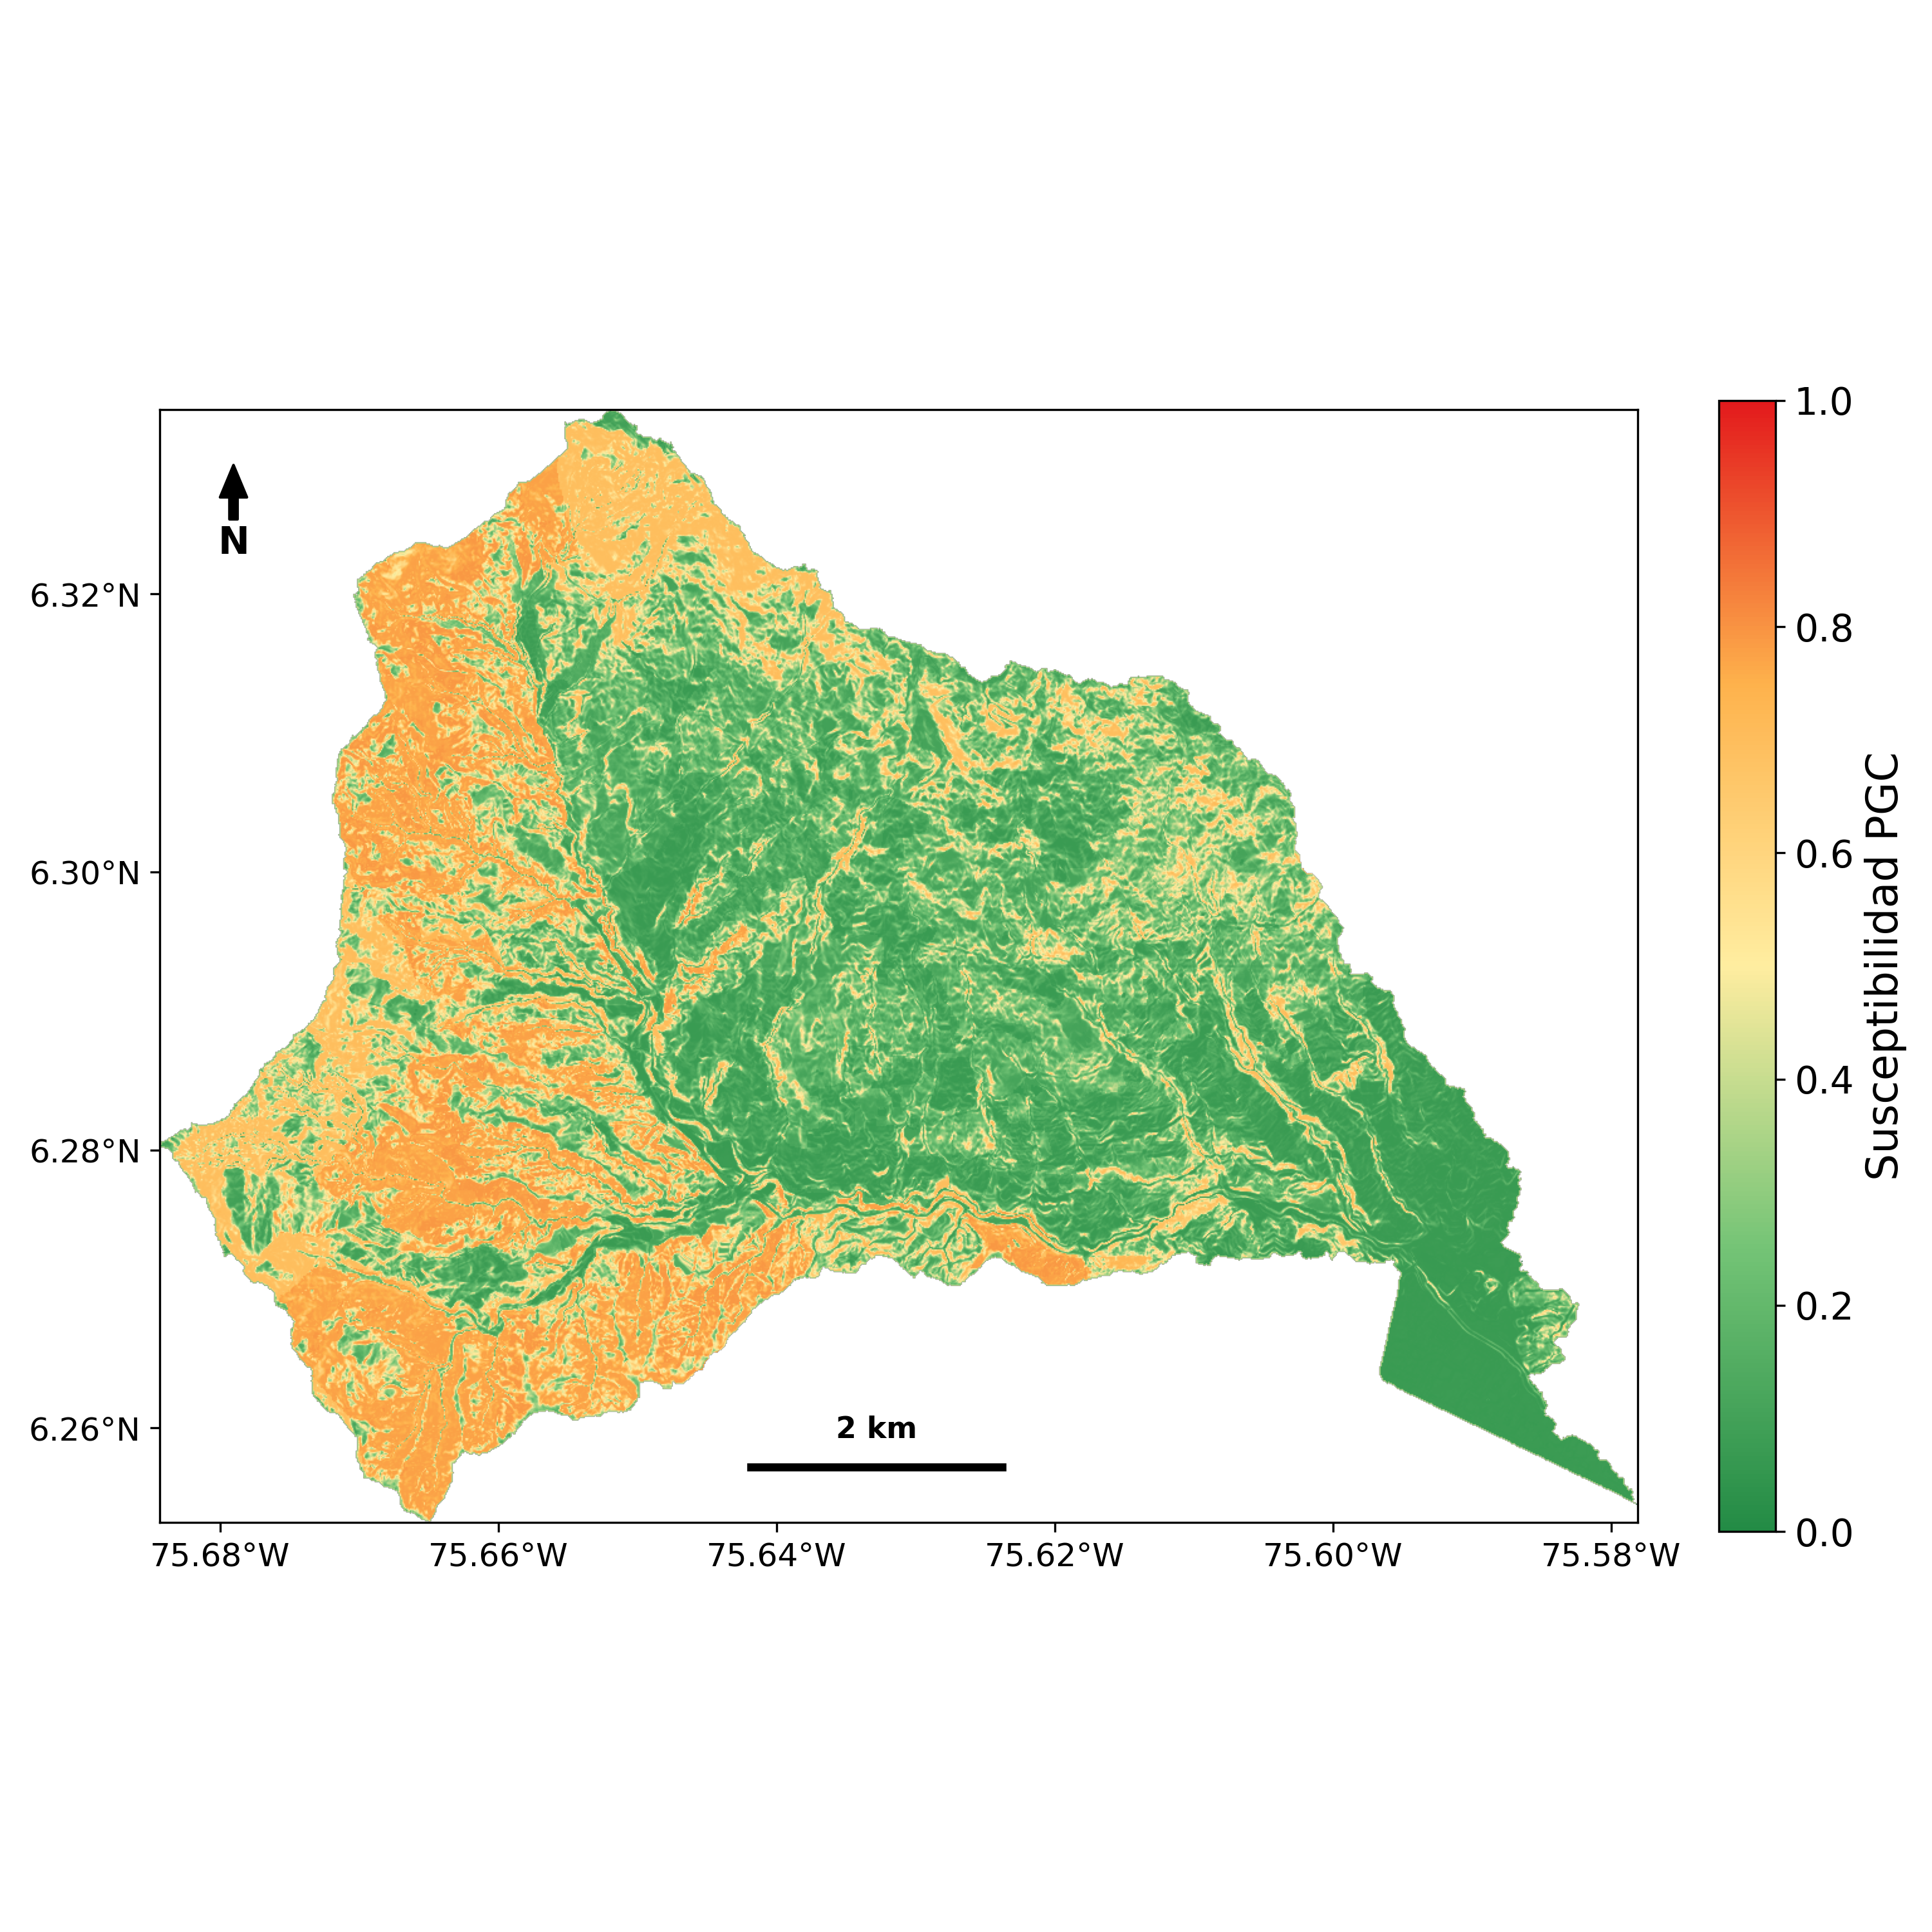
\includegraphics[width=0.85\textwidth]{Fig9_winner_susceptibility.png}
    \caption{Mapa de susceptibilidad del modelo PGC óptimo (pendiente, geología y cobertura). La escala de color varía de verde
    oscuro (muy baja susceptibilidad) a rojo (muy alta susceptibilidad).}
    \label{fig:mapa_final}
\end{figure}

El mapa de incertidumbre del PGC (Fig.~\ref{fig:mapa_std}) muestra la desviación estándar posterior del PGR auxiliar entrenado 
sobre las etiquetas binarias, utilizado como proxy de la incertidumbre epistémica del PGC. Los valores más altos se concentran 
en los extremos de la cuenca y en zonas con escasa cobertura del inventario, mientras que las laderas medias, donde el inventario 
es más denso, presentan la menor incertidumbre.

\begin{figure}[H]
    \centering
    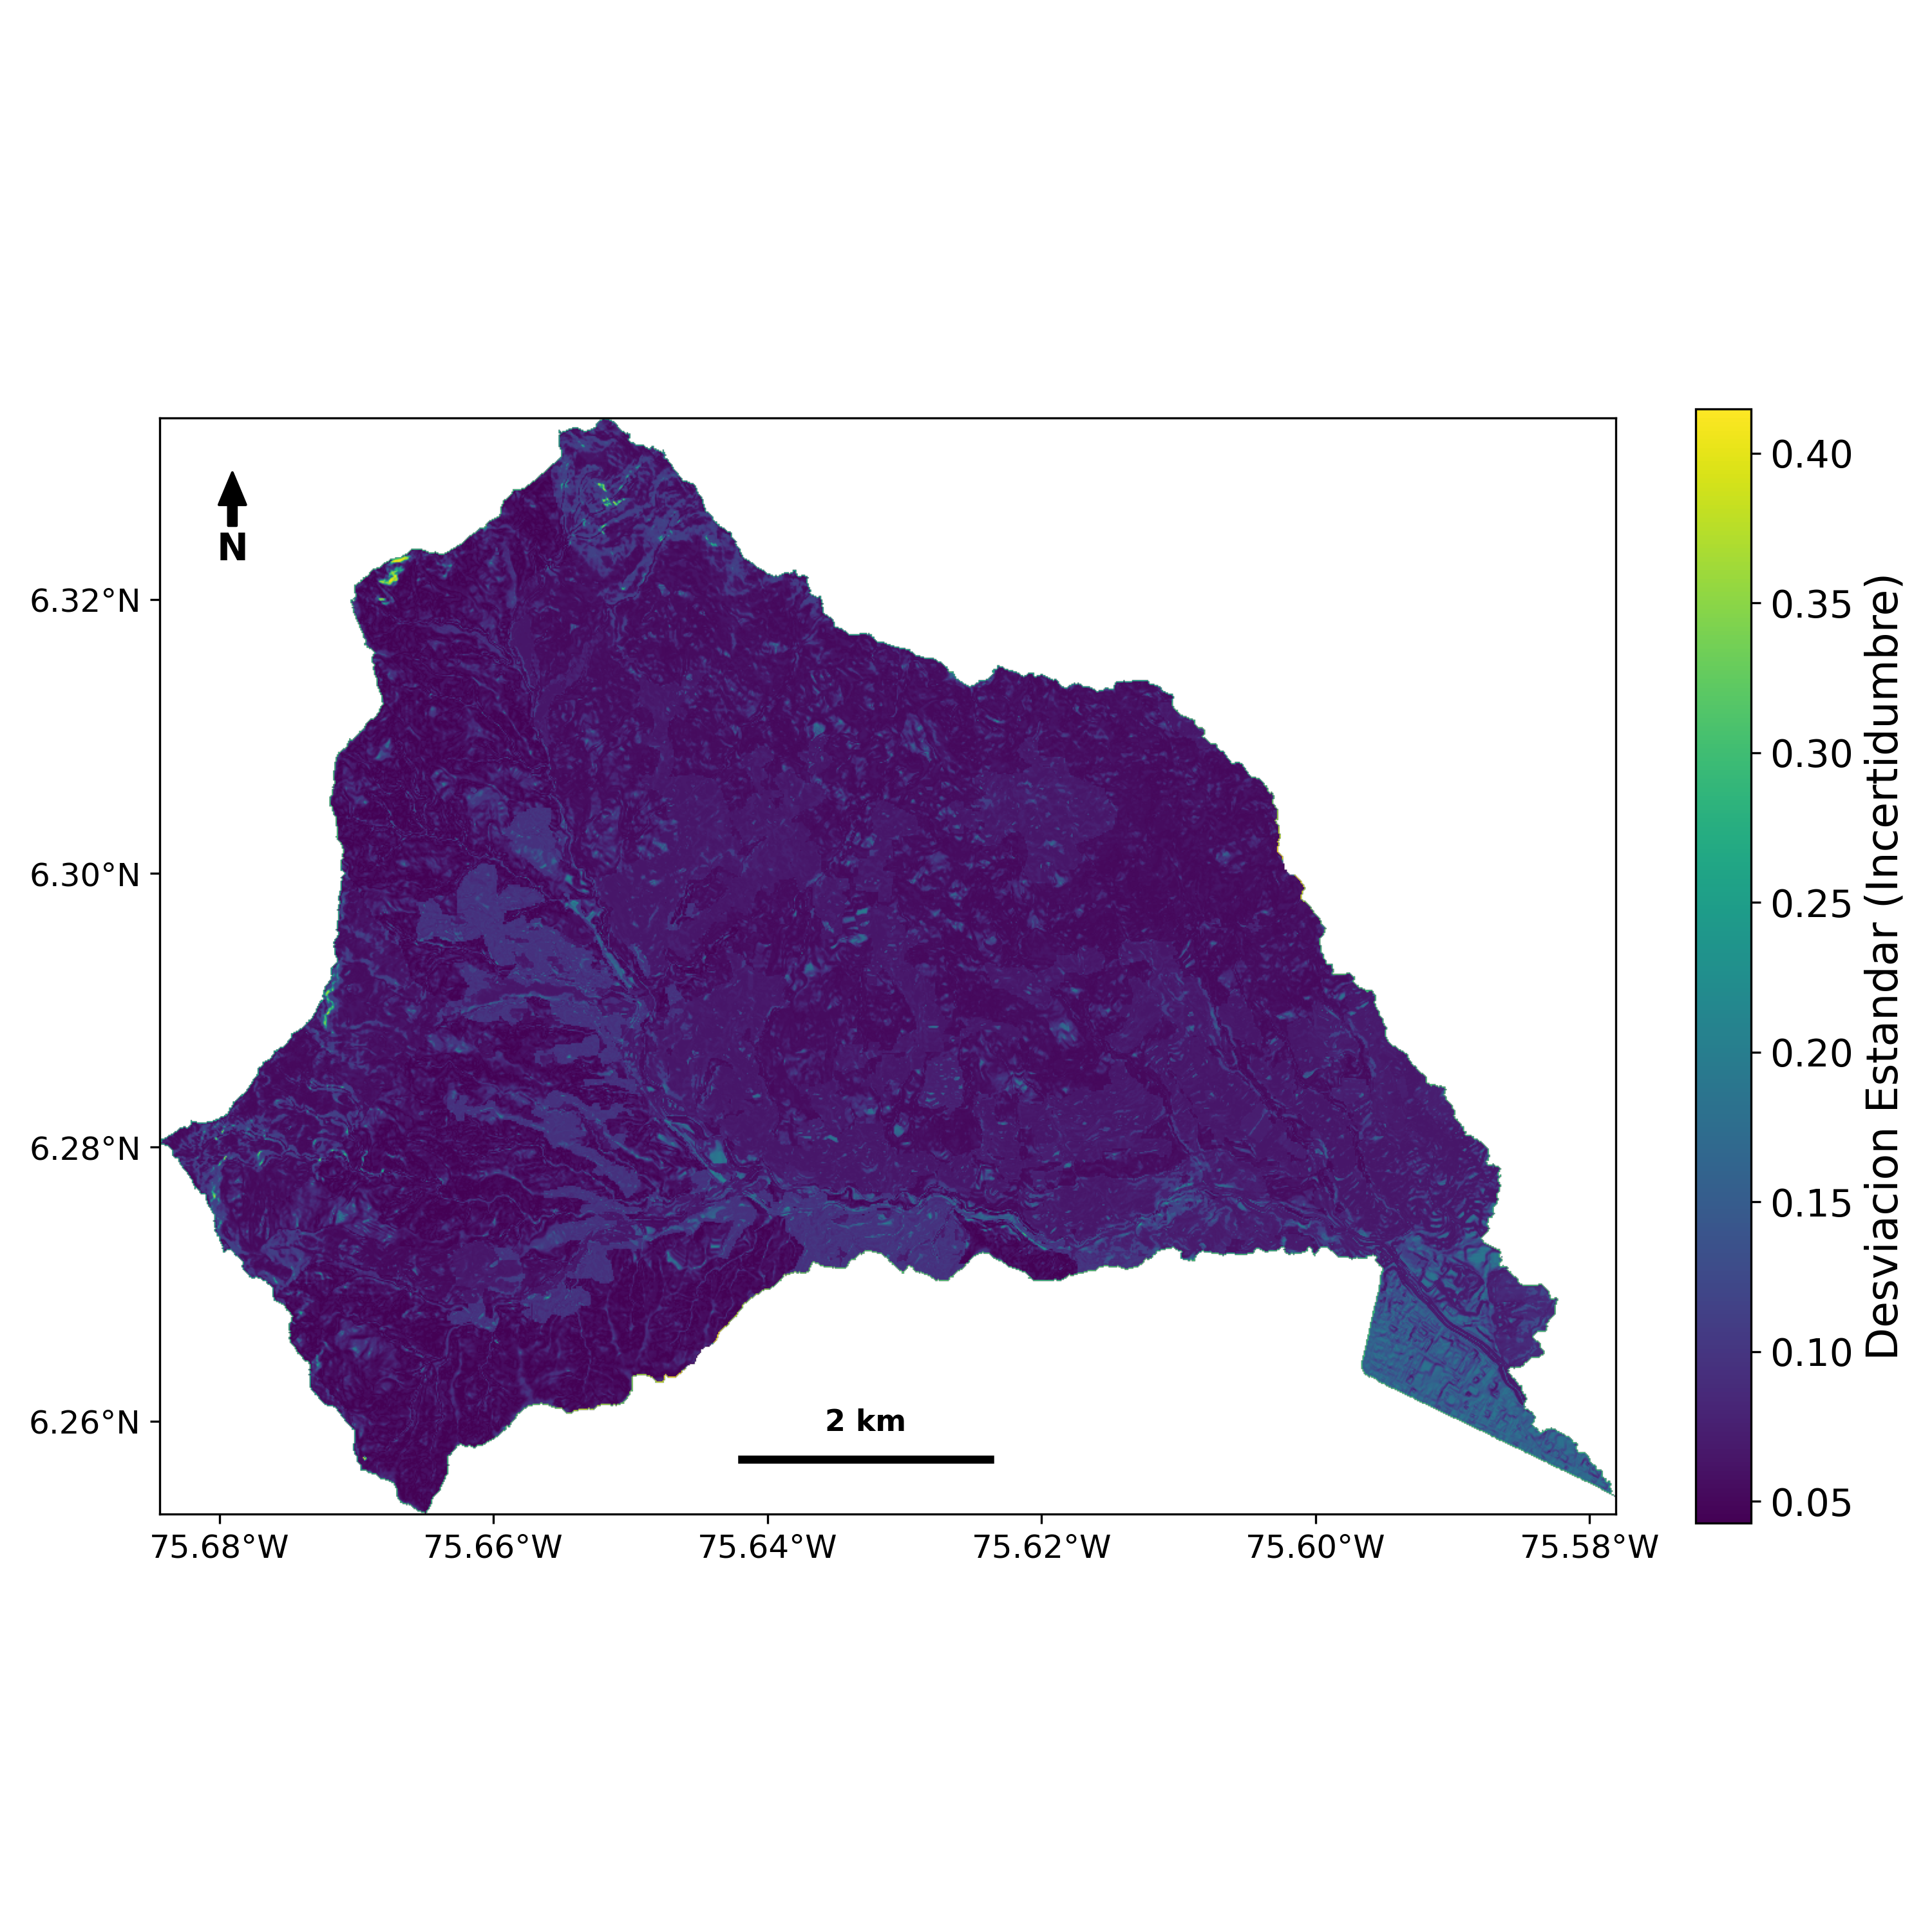
\includegraphics[width=0.85\textwidth]{Fig10_winner_uncertainty.png}
    \caption{Mapa de incertidumbre espacial (desviación estándar posterior del PGR auxiliar sobre etiquetas binarias) del modelo PGC óptimo. 
    Valores altos (amarillo) indican zonas donde la predicción está pobremente restringida por los datos históricos.}
    \label{fig:mapa_std}
\end{figure}

\begin{figure}[H]
    \centering
    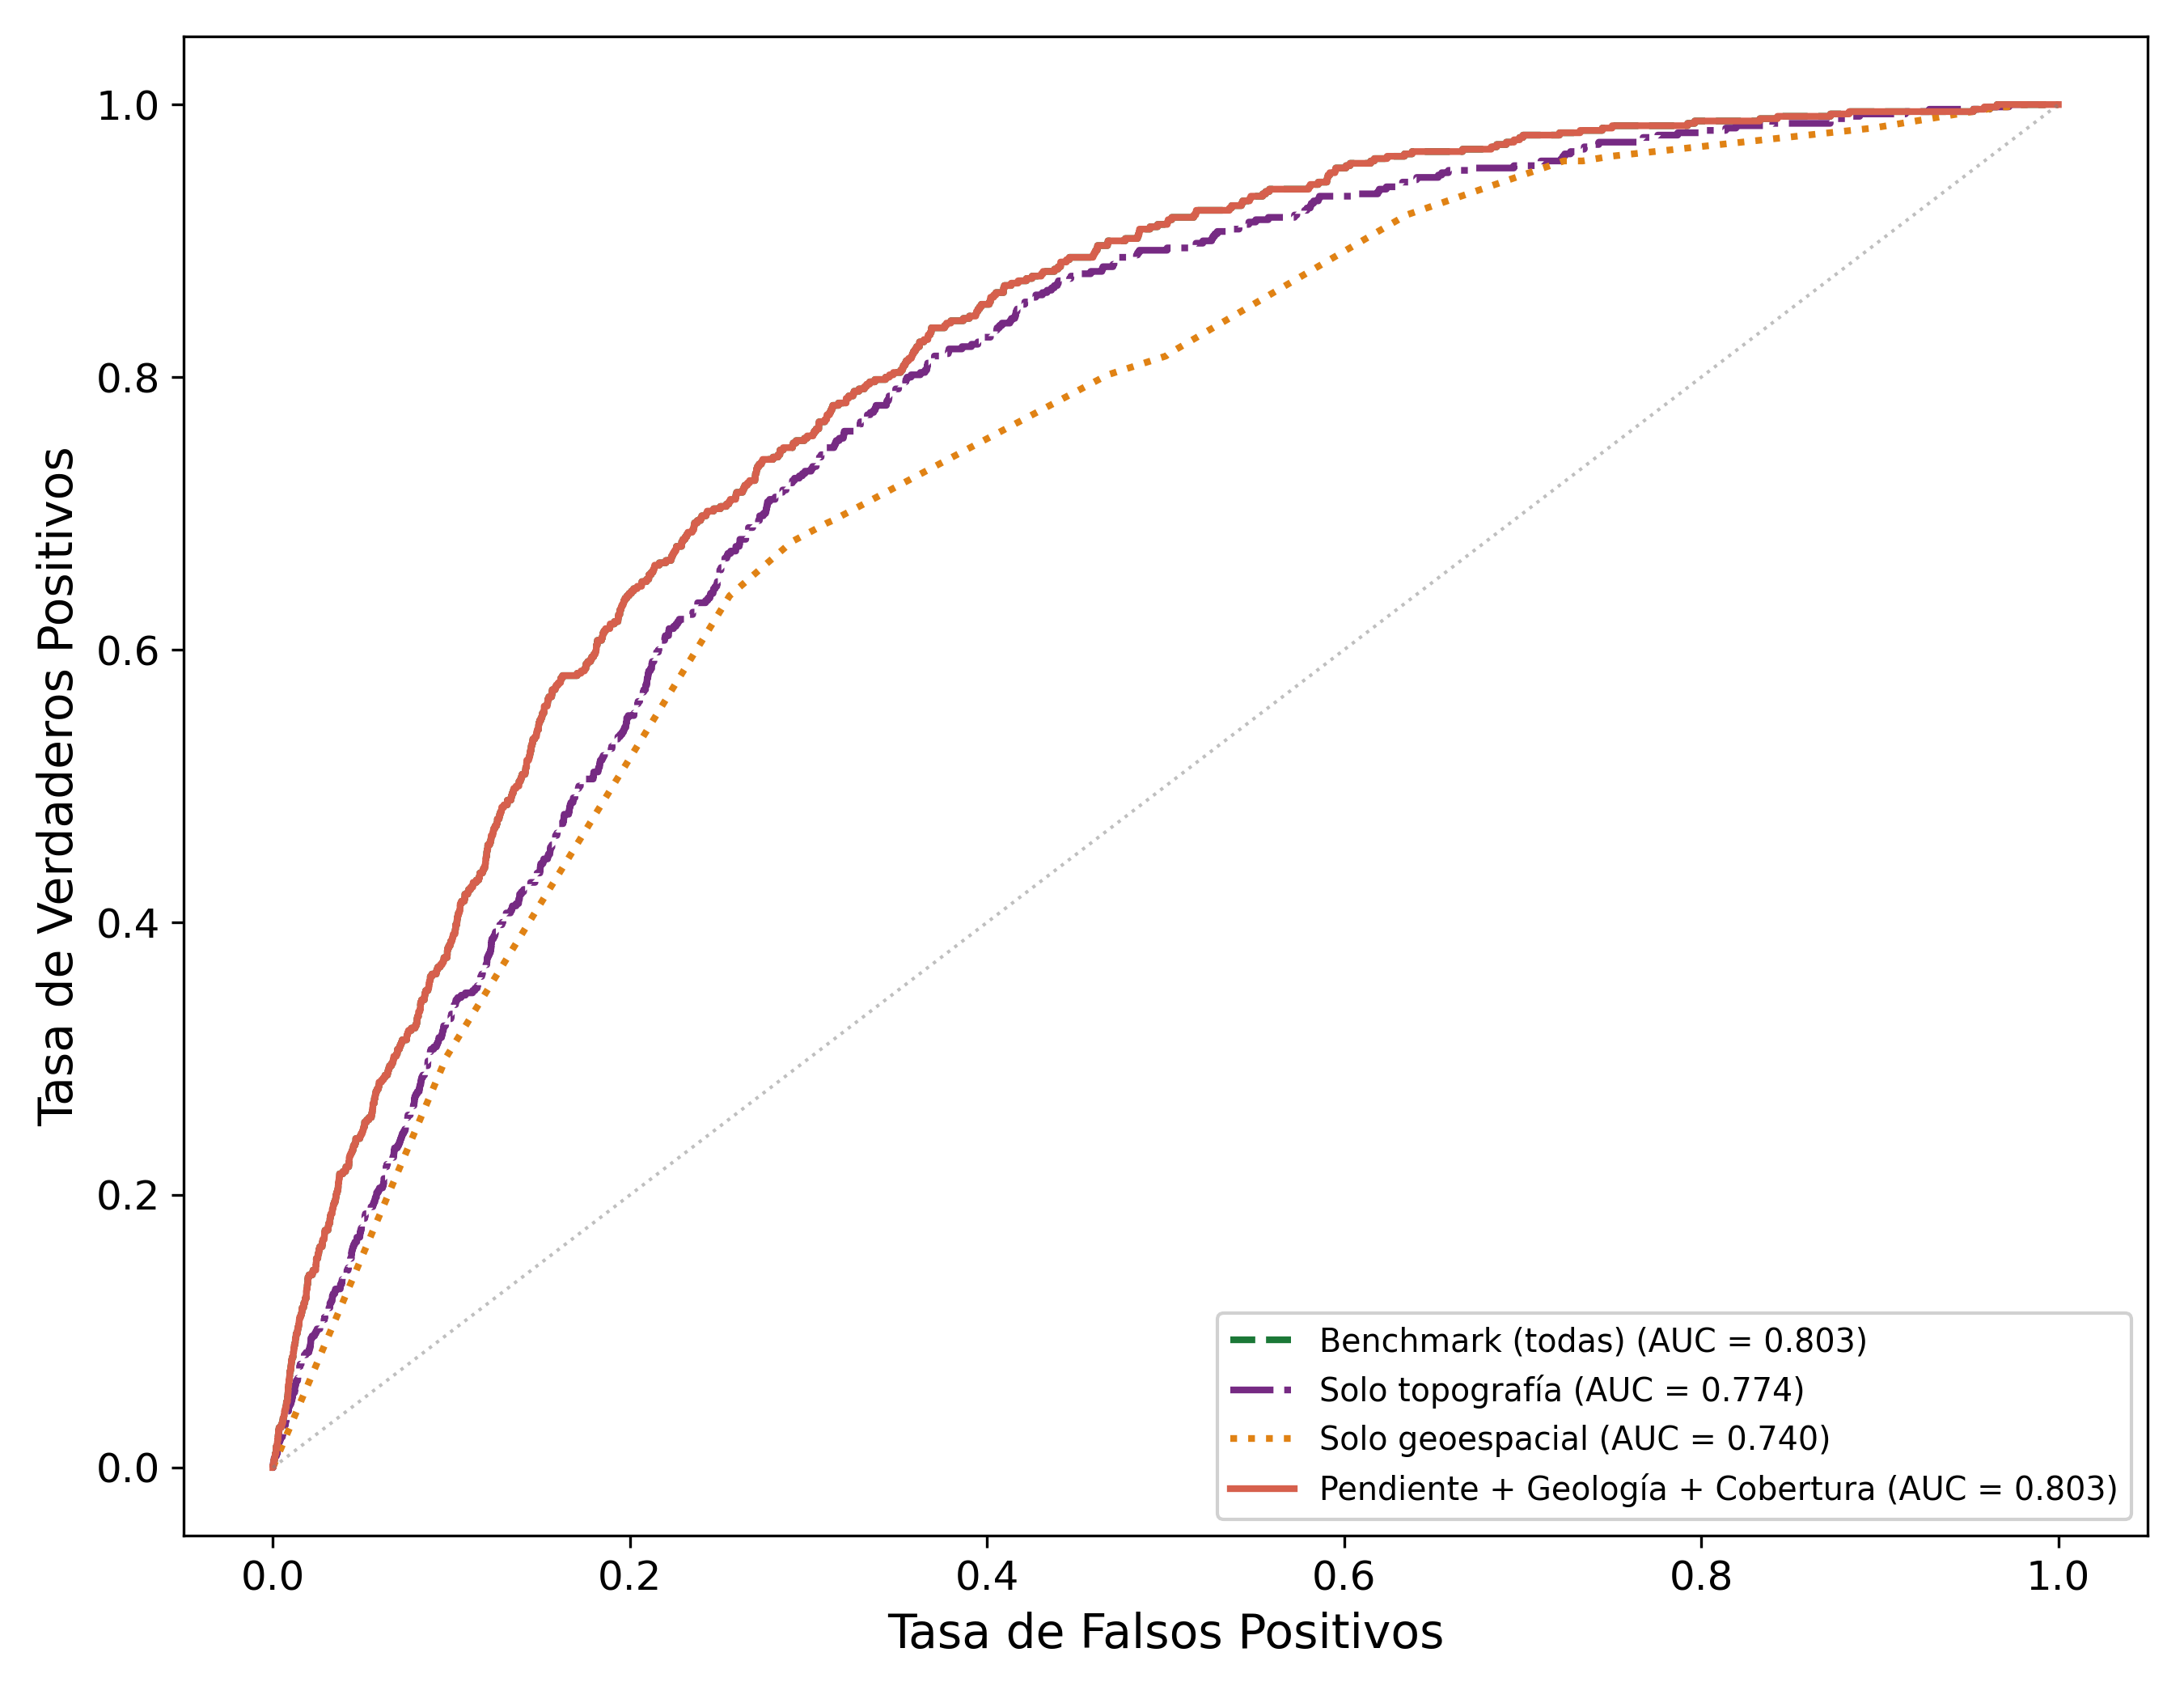
\includegraphics[width=0.72\textwidth]{Fig8_roc_pgc.png}
    \caption{Curvas ROC para las cuatro configuraciones del PGC: \textit{todas las variables}, modelo topográfico 
    puro (pendiente, aspecto, ITH), modelo categoŕico puro (geología, cobertura) y modelo óptimo (pendiente~+~geología~+~cobertura).}
    \label{fig:roc_pgc}
\end{figure}

El análisis ARD del modelo PGC óptimo (Tabla~\ref{tab:ard}) revela que la cobertura del suelo es el factor dominante
(importancia 0{,}272), seguida de la pendiente (0{,}215) y la geología (0{,}062).

\begin{table}[H]
    \centering
    \caption{Importancia relativa de las variables en el modelo PGC óptimo, estimada como el inverso de la longitud 
    de escala ARD optimizada.}
    \label{tab:ard}
    \begin{tabular}{lcc}
        \toprule
        Variable & Longitud de escala ($l_d^*$) & Importancia ($1/l_d^*$) \\
        \midrule
        Cobertura del suelo & 3{,}67 & 0{,}272 \\
        Pendiente & 4{,}65 & 0{,}215 \\
        Geología & 16{,}09 & 0{,}062 \\
        \bottomrule
    \end{tabular}
\end{table}


\section{Discusión}
\label{sec:discusion}

La correlación prácticamente nula entre las predicciones del PGR y la superficie KDE ($r = 0{,}061$) confirma que el espacio de
covariables locales, como pendiente, aspecto e ITH, no tiene capacidad suficiente para predecir la densidad espacial del inventario. 
El PGR podría ser apropiado si el objetivo fuera predecir la densidad regional 
de eventos en un contexto con datos ambientales y morfometricos a escala similar. Para este caso local (escala de celda) los resultados señalan 
que las variables morfometricas no explican adecuadamente la densidad de deslizamientos.

En contraste, el PGC trata cada celda como un ensayo de Bernoulli y optimiza directamente la función latente bajo la verosimilitud 
binaria, garantizando la alineación entre criterio de entrenamiento y evaluación. Esto explica la ganancia de 26 puntos de AUC
respecto al PGR. Para el modelado de susceptibilidad a escala de celda con covariables estáticas del terreno, el PGC indica ser un 
metodo estadísticamente mas apropiado.

La comparación de los modelos univariados en ambos tipos de modelo
(Tablas~\ref{tab:pgr_kde} y~\ref{tab:pgc}) muestra que la jerarquía de importancia de las variables cambia al cambiar el tipo de modelo.
En el PGR, las variables categóricas dominan (geología: AUC~=~0{,}694; cobertura: 0{,}631), mientras que la pendiente es la menos
informativa (0{,}543). En el PGC, la cobertura del suelo es el predictor más relevante (importancia ARD~=~0{,}272),
seguida de la pendiente (0{,}215) y la geología (0{,}062). Esto podria tambien explicarse por la escala de analisis que explica cada modelo.
Las variables morfometricas explican condiciones locales o puntuales, lo que se alinea mejor con el modelo PGC binario que representa
la probabilida de Bernoulli de la presencia de un deslizamiento. Mientras que la superficie del modelo PGR es una densidad que representa 
una condicion regional y no puntual, que al parecer es explicada por variables regionales.

Esta diferencia refleja la escala de los dos objetivos de predicción. El ancho de banda KDE
($h \approx 691$~m) suaviza el inventario en una ventana de más de medio kilómetro, de modo que la variable de respuesta del
PGR captura la recurrencia regional de eventos. Las unidades geológicas y de cobertura del suelo, cuya extensión espacial supera
frecuentemente los 691~m, son buenos predictores de la densidad regional del inventario precisamente porque sus límites coinciden
con las concentraciones suavizadas de eventos. La pendiente, en cambio, varía a la escala del píxel (5~m) y no tiene correlación
sistemática con la vecindad KDE. En el PGC, el objetivo es discriminar celdas individuales; a esta resolución, la cobertura
del suelo emerge como el predictor dominante, superando a la pendiente, lo que indica que las variaciones locales de la cobertura, 
que en la cuenca La Iguana reflejan directamente la urbanización informal y la intervencion antropica en ladera, son el factor
condicionante con mayor capacidad discriminativa. Este contraste indica que la importancia de una variable no es al parecer una propiedad
intrínseca de la covariable, sino dependiente de la escala espacial.

Los resultados indican que el PG alcanza un desempeño competitivo con pocas variables y proporciona como producto nativo la distribución posterior 
completa sobre la susceptibilidad. Desde una perspectiva práctica, un modelo parsimonioso tiene implicaciones directas para 
la transferibilidad del método a cuencas con recursos limitados de datos. 

La Fig.~\ref{fig:uncertainty_cov} ilustra cómo se estructura la incertidumbre en el espacio de las tres variables del modelo
óptimo (pendiente, geología y cobertura). Para la pendiente (panel~A), la desviación estándar posterior es mínima en el rango
20°--45°, que concentra la mayor densidad del inventario de entrenamiento, y aumenta hacia los extremos, donde el modelo
extrapola. Para las variables categóricas (paneles~B y~C), las diferencias inter-clase reflejan la heterogeneidad interna de
cada unidad y su representación en el conjunto de entrenamiento.

\begin{figure}[H]
    \centering
    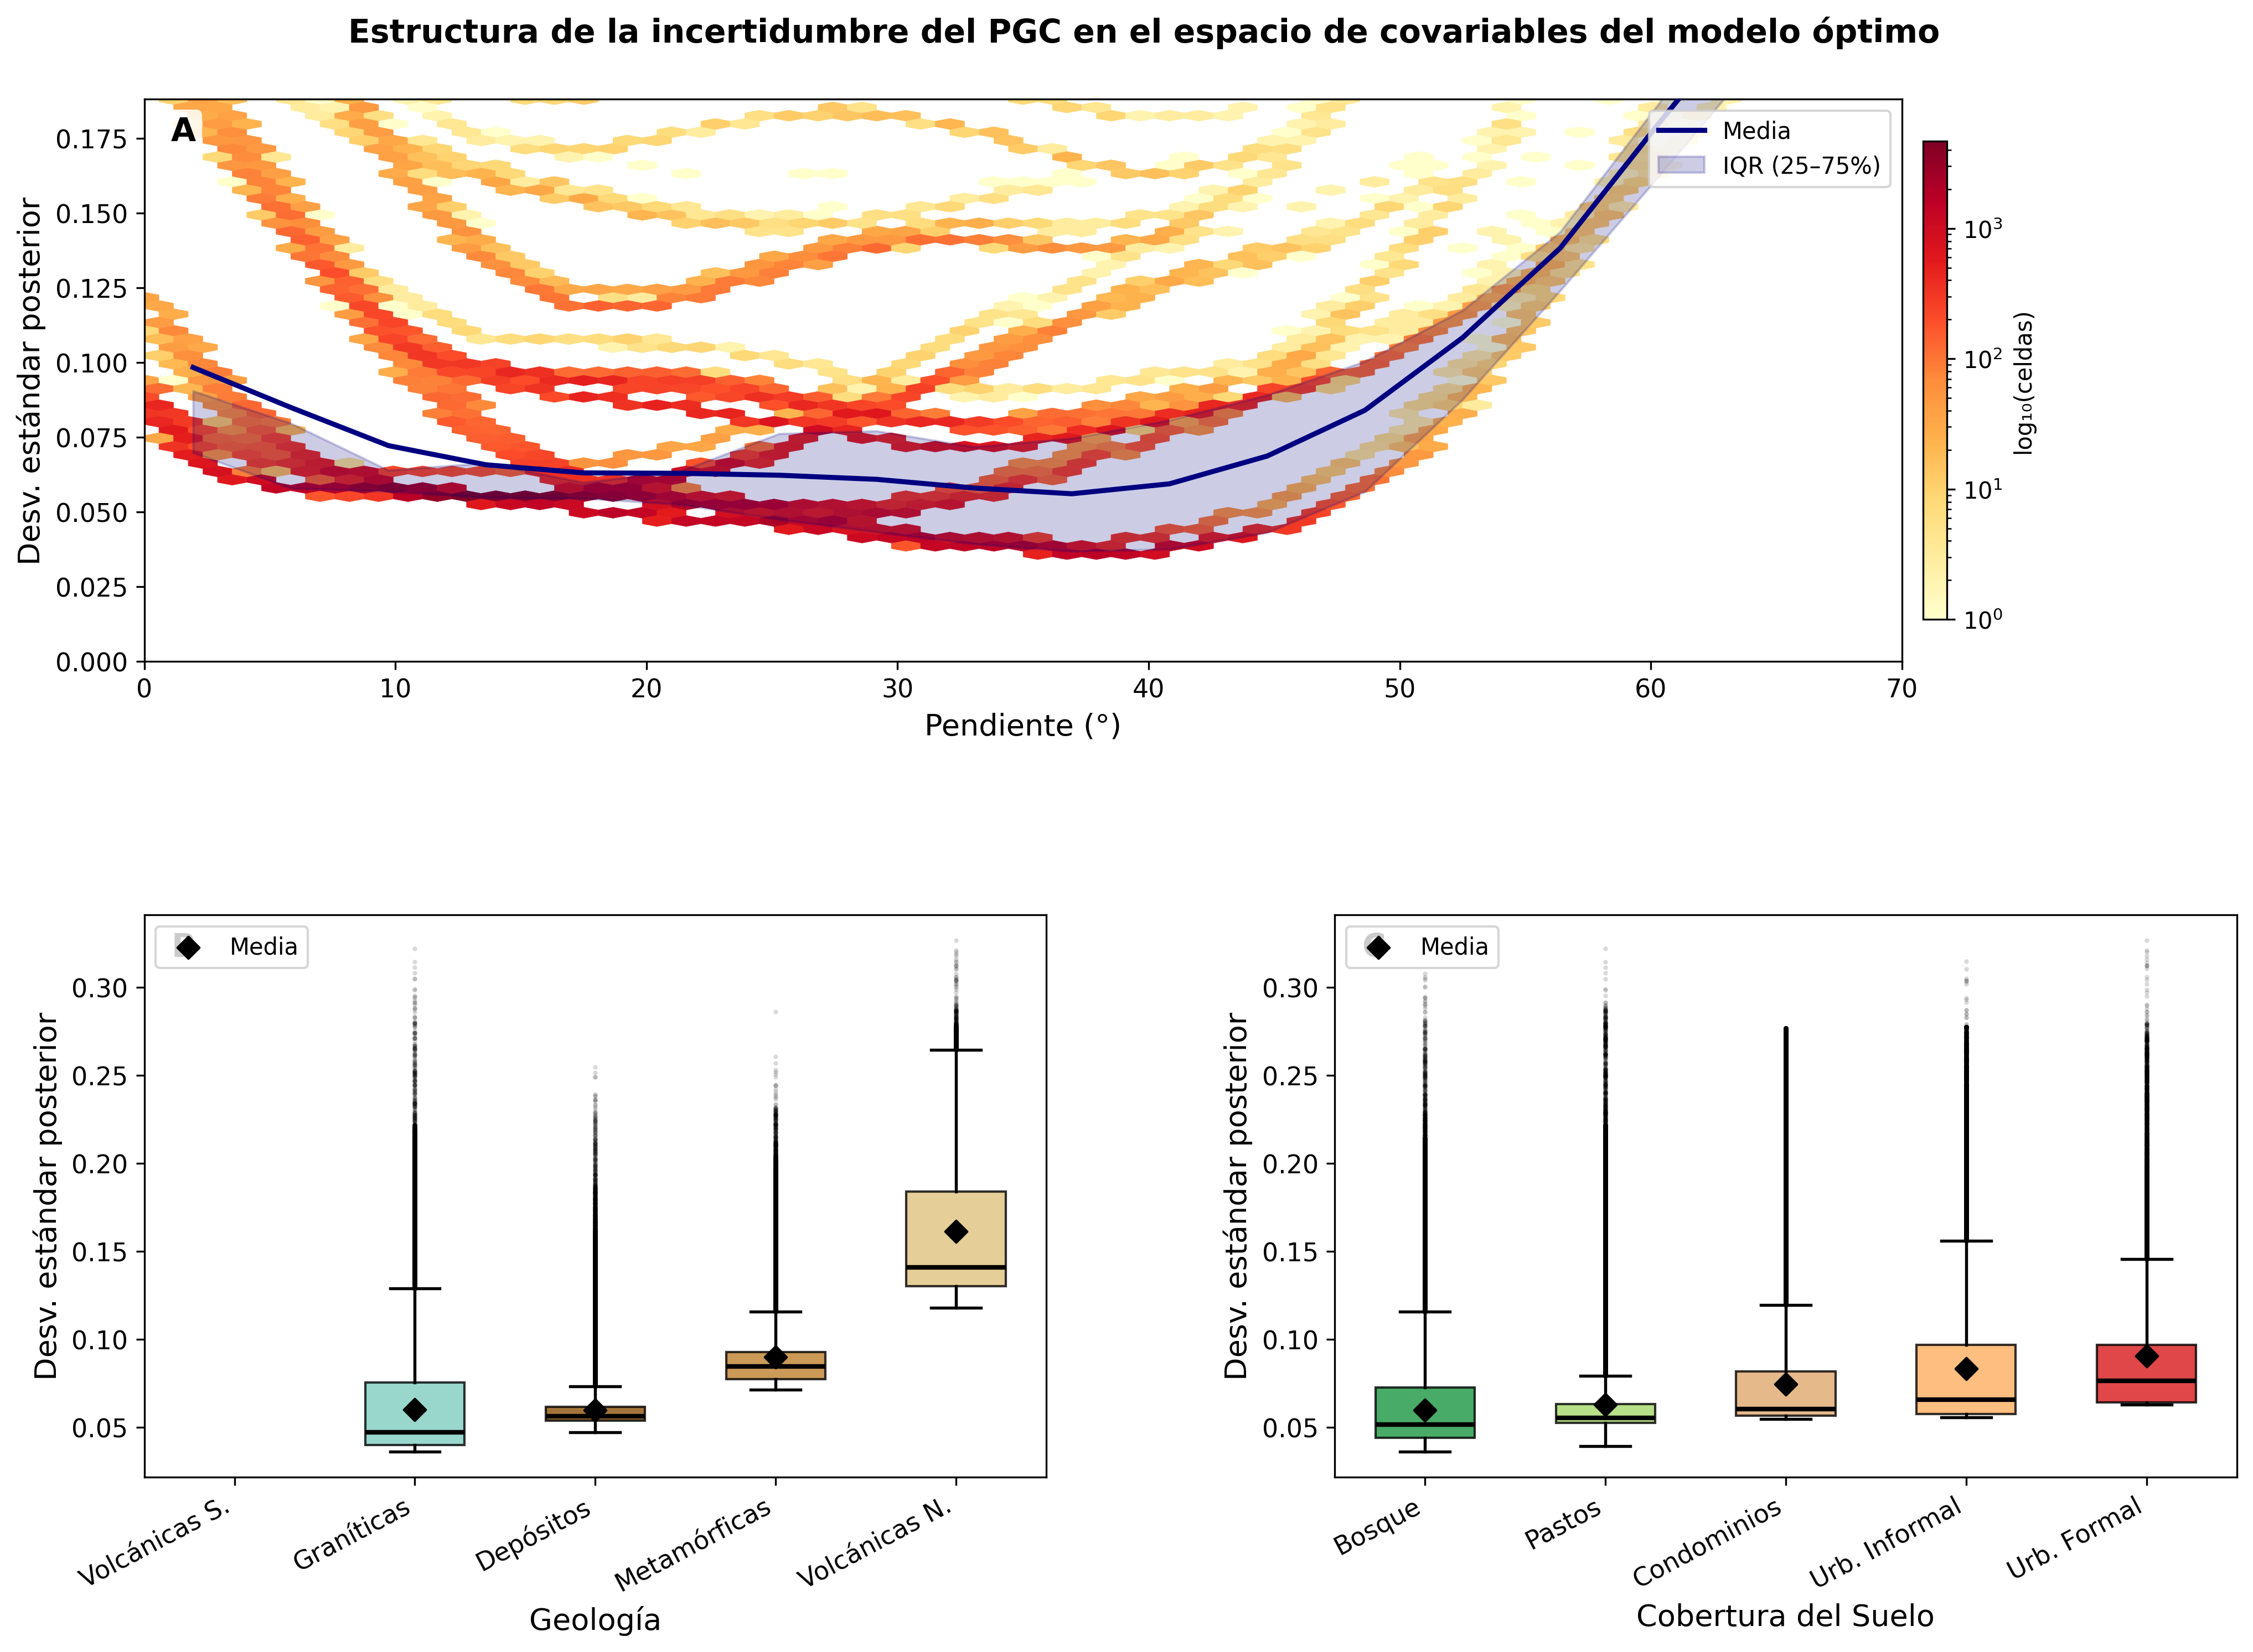
\includegraphics[width=1.0\textwidth]{Fig11_uncertainty_covariates.png}
    \caption{Incertidumbre del PGC (desviación estándar posterior) en el espacio de las tres variables del modelo óptimo.
    Panel~A: hexbin (densidad logarítmica) con media binada (línea azul) e IQR~(25--75\%) como función de la pendiente;
    la forma cóncava confirma que la menor incertidumbre se concentra en el rango 20°--45°.
    Panel~B: boxplots por unidad geológica. Panel~C: boxplots por clase de cobertura del suelo.}
    \label{fig:uncertainty_cov}
\end{figure}


La Fig.~\ref{fig:uncertainty_class} examina la relación continua entre la susceptibilidad predicha y la incertidumbre
para el PGC. La desviación estándar posterior presenta una tendencia decreciente a medida que aumenta la susceptibilidad:
las celdas con probabilidad alta ($> 0{,}6$) tienen la menor incertidumbre, indicando que corresponden a combinaciones de
covariables bien representadas en el inventario y son, por tanto, las más robustamente identificadas para la priorización
de medidas de mitigación.

\begin{figure}[H]
    \centering
    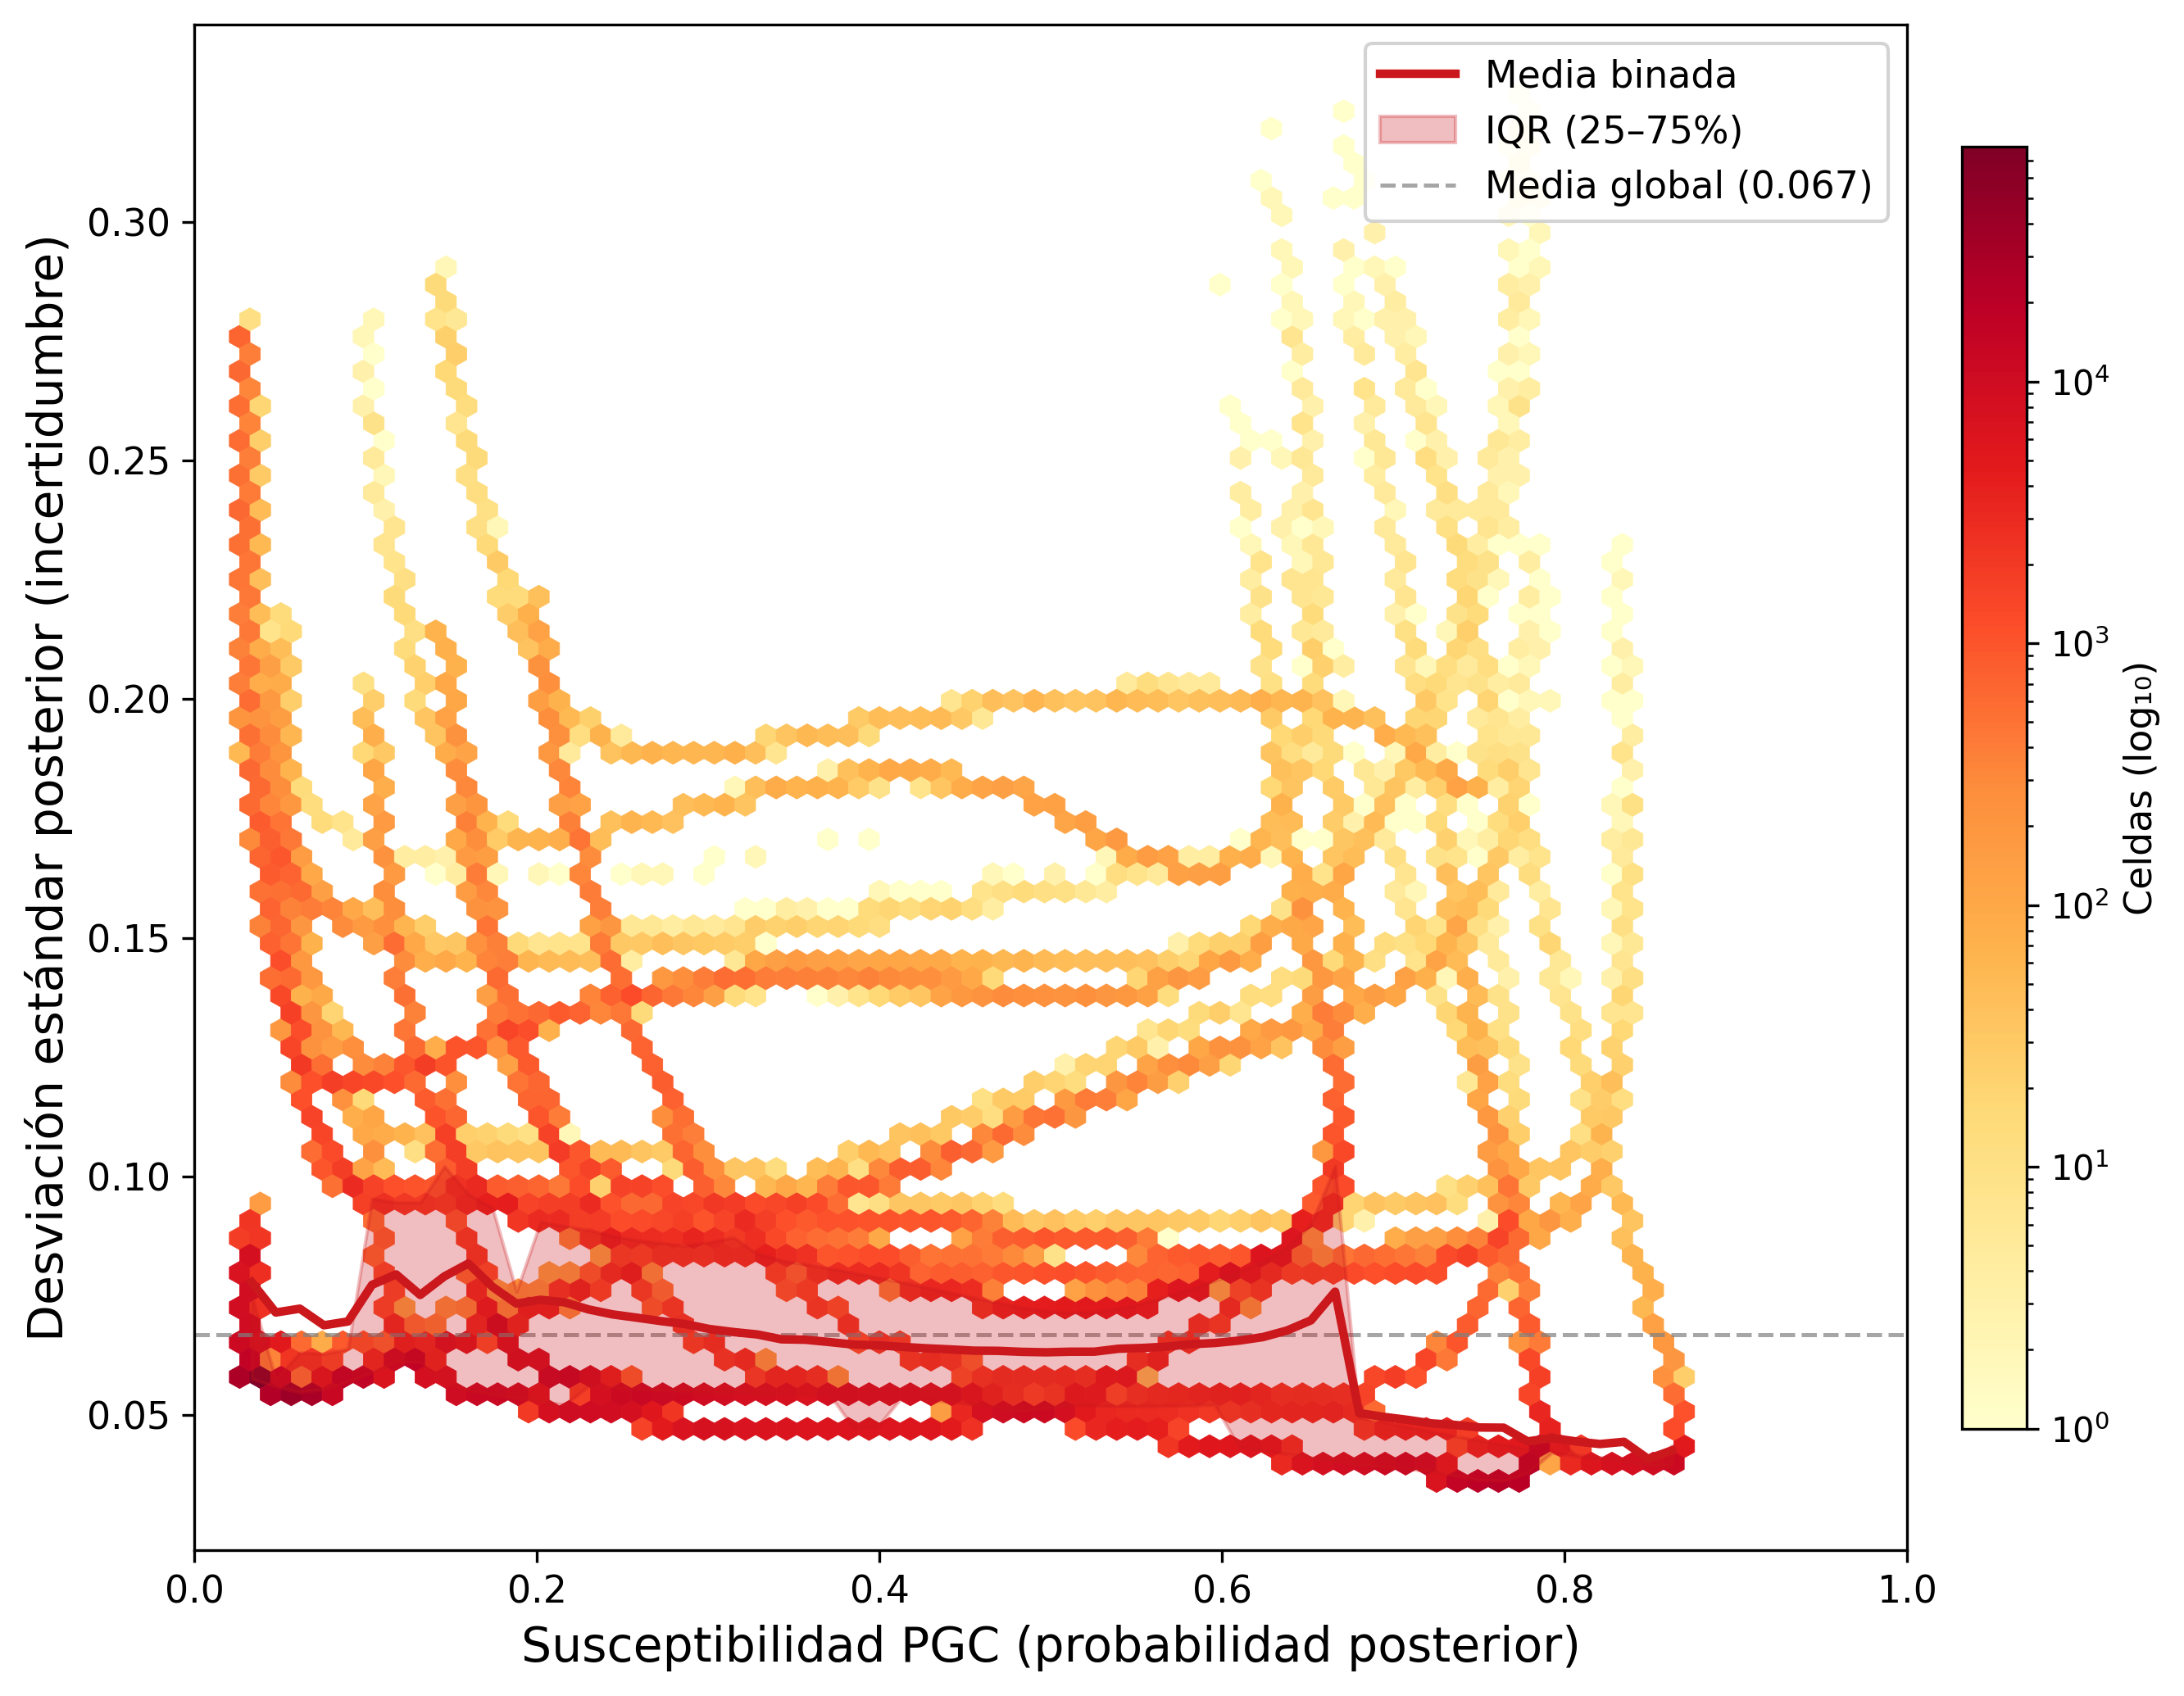
\includegraphics[width=0.75\textwidth]{Fig12_uncertainty_vs_susceptibility.png}
    \caption{Incertidumbre del PGC (desviación estándar posterior) como función continua de la susceptibilidad predicha.
    Se muestran las 2{,}087{,}643~celdas de la cuenca como hexbin (densidad en escala logarítmica), la media binada
    (línea roja) y el rango intercuartílico IQR~25--75\% (banda sombreada). La incertidumbre decrece con la susceptibilidad,
    lo que indica que las zonas de alta susceptibilidad están mejor restringidas por los datos de entrenamiento.}
    \label{fig:uncertainty_class}
\end{figure}

La combinación de susceptibilidad media e incertidumbre permite una clasificación bidimensional del territorio en cuatro 
categorías accionables: (i)~alta susceptibilidad y baja incertidumbre, zonas prioritarias para inversión en mitigación; 
(ii)~alta susceptibilidad y alta incertidumbre, zonas que requieren validación de campo; (iii)~baja susceptibilidad y 
baja incertidumbre, zonas razonablemente seguras; y (iv)~baja susceptibilidad y alta incertidumbre, zonas donde ampliar 
el inventario histórico reduciría la varianza posterior del modelo. Esta clasificación bidimensional es cualitativamente 
superior a la que proporciona cualquier método sin cuantificación de incertidumbre.

El marco propuesto presenta limitaciones a considerar. El conjunto de entrenamiento de 500 puntos representa el 0{,}024\% de 
las celdas válidas; estrategias de muestreo espacialmente
estratificado podrían mejorar la representatividad y reducir el sesgo asociado al desequilibrio de clases
\citep{Heckmann2014, Chawla2002}. El \textit{target encoding} \citep{MicciBarreca2001} calculado sobre el conjunto completo de
datos introduce riesgo de filtración de información; implementaciones más rigurosas lo calcularían mediante validación cruzada.
El modelo no captura explícitamente la autocorrelación espacial residual \citep{Lombardo2018}, lo que puede inflar la capacidad
discriminativa aparente medida por el AUC-ROC \citep{Fawcett2006}.

\section{Conclusiones}
\label{sec:conclusiones}

Una de las contribuciones más relevantes de los modelos de Procesos Gaussianos frente a los enfoques clásicos de aprendizaje
automático ---como la regresión logística, los bosques aleatorios o las máquinas de soporte vectorial--- reside en su capacidad
para representar la susceptibilidad como una superficie continua y probabilística en el espacio de las covariables. Mientras
que los modelos convencionales producen una estimación puntual de la probabilidad de ocurrencia, los PG proporcionan, para cada
celda del territorio, una distribución posterior completa sobre dicha probabilidad. Esto permite cuantificar de forma rigurosa la
incertidumbre asociada a cada predicción, reconociendo explícitamente que la información histórica de inventarios
puede no cubrir uniformemente todo el terreno.

Esta capacidad de incertidumbre cuantificada se materializa en el mapa de desviación estándar posterior, que identifica
objetivamente las zonas donde la predicción está pobremente restringida por los datos históricos. La distinción entre zonas de
alta susceptibilidad con baja incertidumbre ---prioritarias para medidas inmediatas de mitigación--- y zonas de alta incertidumbre
---que demandan nuevos datos de campo para reducir la ambigüedad del modelo--- convierte al mapa de incertidumbre en una herramienta
fundamental para la toma de decisiones en la gestión territorial del riesgo de desastres, información que los modelos clásicos simplemente
no pueden proveer.

Finalmente, el análisis ARD evidencia un marcado cambio en la importancia relativa de las variables condicionantes en función
de la escala de análisis. A la resolución de 5~m adoptada en este estudio, la cobertura del suelo emerge como el factor dominante
(importancia~=~0{,}272), superando a la pendiente (0{,}215) y distanciándose notablemente de la geología (0{,}062). Este resultado
contrasta con la jerarquía de variables propia de estudios regionales o de menor resolución, donde los factores geomorfológicos
y litológicos suelen predominar. A escala de celda, la intervención antrópica del suelo, expresada en las categorías de cobertura
que reflejan urbanización, vegetación degradada o suelos desnudos, captura condicionantes locales de la inestabilidad que se
diluyen en agregaciones espaciales más gruesas, sugiriendo que la importancia de los predictores no es intrínseca sino
dependiente de la escala de observación.


\section*{Financiamiento}
Esta investigación no recibió financiamiento externo.

\section*{Disponibilidad de datos y código}
El código Python y los datos raster necesarios para reproducir el análisis están disponibles en el material suplementario asociado
a este artículo.

\section*{Conflicto de intereses}
El autor declara no tener conflicto de intereses.


%%---------------- BIBLIOGRAFIA --------------------------%%
\hypersetup{urlcolor=blue2}
\renewcommand{\refname}{Referencias}
\renewcommand{\baselinestretch}{1.2}
\small
\begin{thebibliography}{}

\bibitem{Varnes1978} D.J. Varnes, ``Slope movement types and processes,'' {\it Special Report, Transportation Research Board, National Academy of Sciences}, vol. 176, pp. 11--33, 1978.
$\uparrow$\par

\bibitem{Hungr2014} O. Hungr, S. Leroueil, and L. Picarelli, ``The Varnes classification of landslide types, an update,'' {\it Landslides}, vol. 11, no. 2, pp. 167--194, 2014.
\url{https://doi.org/10.1007/s10346-013-0436-y}
$\uparrow$\par

\bibitem{Gomez2023} D. Gómez, E.F. García, and E. Aristizábal, ``Spatial and temporal landslide distributions using global and open landslide databases,'' {\it Natural Hazards}, vol. 117, no. 1, pp. 25--55, 2023.
\url{https://doi.org/10.1007/s11069-023-05848-8}
$\uparrow$\par

\bibitem{Aristizabal2012} E. Aristizábal, H. González, and C. Henriques, ``Analysis of landslides triggered by the October 2007 heavy rains in La Gabriela, Bello, Antioquia, Colombia,'' {\it Landslides}, vol. 9, no. 3, pp. 343--353, 2012.
\url{https://doi.org/10.1007/s10346-011-0311-5}
$\uparrow$\par

\bibitem{Nieto2025} S. Nieto, E. Aristizábal, and U. Ozturk, ``Coupled evolution of a city and landslides,'' {\it Environmental Research Letters}, vol. 20, no. 5, art. 054001, 2025.
\url{https://doi.org/10.1088/1748-9326/adc4d8}
$\uparrow$\par

\bibitem{Klimes2010} J. Klimeš and M. Rios Escobar, ``A landslide susceptibility assessment in urban areas based on existing data: an example from the Iguaná Valley, Medellín City, Colombia,'' {\it Natural Hazards and Earth System Sciences}, vol. 10, no. 10, pp. 2067--2079, 2010.
\url{https://doi.org/10.5194/nhess-10-2067-2010}
$\uparrow$\par

\bibitem{Guzzetti2005} F. Guzzetti, P. Reichenbach, F. Ardizzone, M. Cardinali, and M. Galli, ``Estimating the quality of landslide susceptibility models,'' {\it Geomorphology}, vol. 81, no. 1--2, pp. 166--184, 2005.
\url{https://doi.org/10.1016/j.geomorph.2006.04.007}
$\uparrow$\par

\bibitem{Corominas2014} J. Corominas {\it et al.}, ``Recommendations for the quantitative analysis of landslide risk,'' {\it Bulletin of Engineering Geology and the Environment}, vol. 73, no. 2, pp. 209--263, 2014.
\url{https://doi.org/10.1007/s10064-013-0538-8}
$\uparrow$\par

\bibitem{Reichenbach2018} P. Reichenbach, M. Rossi, B.D. Malamud, M. Mihir, and F. Guzzetti, ``A review of statistically-based landslide susceptibility models,'' {\it Earth-Science Reviews}, vol. 180, pp. 60--91, 2018.
\url{https://doi.org/10.1016/j.earscirev.2018.03.001}
$\uparrow$\par

\bibitem{Chen2017} W. Chen {\it et al.}, ``A comparative study of logistic model tree, random forest, and classification and regression tree models for spatial prediction of landslide susceptibility,'' {\it Catena}, vol. 151, pp. 147--160, 2017.
\url{https://doi.org/10.1016/j.catena.2016.11.032}
$\uparrow$\par

\bibitem{HosmerLemeshow2000} D.W. Hosmer and S. Lemeshow, {\it Applied Logistic Regression}, 2nd ed. John Wiley \& Sons, New York, 2000.
\url{https://doi.org/10.1002/0471722146}
$\uparrow$\par

\bibitem{Atkinson1998} P.M. Atkinson and R. Massari, ``Generalised linear modelling of susceptibility to landsliding in the central Apennines, Italy,'' {\it Computers \& Geosciences}, vol. 24, no. 4, pp. 373--385, 1998.
\url{https://doi.org/10.1016/S0098-3004(97)00117-9}
$\uparrow$\par

\bibitem{Fawcett2006} T. Fawcett, ``An introduction to ROC analysis,'' {\it Pattern Recognition Letters}, vol. 27, no. 8, pp. 861--874, 2006.
\url{https://doi.org/10.1016/j.patrec.2005.10.010}
$\uparrow$\par

\bibitem{VanWesten2003} C.J. van Westen, N. Rengers, and R. Soeters, ``Use of geomorphological information in indirect landslide susceptibility assessment,'' {\it Natural Hazards}, vol. 30, no. 3, pp. 399--419, 2003.
\url{https://doi.org/10.1023/B:NHAZ.0000007097.42735.9e}
$\uparrow$\par

\bibitem{Heckmann2014} T. Heckmann, K. Gegg, A. Gegg, and M. Becht, ``Sample size matters: investigating the effect of sample size on a logistic regression susceptibility model for debris flows,'' {\it Natural Hazards and Earth System Sciences}, vol. 14, no. 2, pp. 259--278, 2014.
\url{https://doi.org/10.5194/nhess-14-259-2014}
$\uparrow$\par

\bibitem{Lombardo2020} L. Lombardo, T. Opitz, F. Ardizzone, F. Guzzetti, and R. Huser, ``Space-time landslide predictive modelling,'' {\it Earth-Science Reviews}, vol. 209, art. 103318, 2020.
\url{https://doi.org/10.1016/j.earscirev.2020.103318}
$\uparrow$\par

\bibitem{Rasmussen2006} C.E. Rasmussen and C.K.I. Williams, {\it Gaussian Processes for Machine Learning}. MIT Press, Cambridge, MA, 2006.
\url{http://www.gaussianprocess.org/gpml/}
$\uparrow$\par

\bibitem{Gao2021} Z. Gao {\it et al.}, ``Landslide risk assessment of high-mountain settlements using Gaussian process classification combined with improved weight-based generalized objective function,'' {\it International Journal of Disaster Risk Reduction}, vol. 67, art. 102662, 2021.
\url{https://doi.org/10.1016/j.ijdrr.2021.102662}
$\uparrow$\par

\bibitem{Cheng2022} C. Cheng, Y. Yang, F. Zhong, C. Song, and Y. Zhen, ``An optimization of statistical index method based on Gaussian process regression and GeoDetector, for higher accurate landslide susceptibility modeling,'' {\it Applied Sciences}, vol. 12, no. 20, art. 10196, 2022.
\url{https://doi.org/10.3390/app122010196}
$\uparrow$\par

\bibitem{Yang2022} W. Yang, Y. Feng, J. Wan, and L. Wang, ``Sparse Gaussian process regression for landslide displacement time-series forecasting,'' {\it Frontiers in Earth Science}, vol. 10, art. 944301, 2022.
\url{https://doi.org/10.3389/feart.2022.944301}
$\uparrow$\par

\bibitem{AristizabalYokota2008} E. Aristizábal and S. Yokota, ``Evolución geomorfológica del Valle de Aburrá y sus implicaciones en la ocurrencia de movimientos en masa,'' {\it Boletín de Ciencias de la Tierra}, vol. 24, pp. 5--18, 2008.
\url{https://revistas.unal.edu.co/index.php/rbct/article/view/9268}
$\uparrow$\par

\bibitem{GarciaDelgado2020} H. García-Delgado and F. Velandia, ``Tectonic geomorphology of the Serranía de San Lucas (Central Cordillera): Regional implications for active tectonics and drainage rearrangement in the Northern Andes,'' {\it Geomorphology}, vol. 349, art. 106914, 2020.
\url{https://doi.org/10.1016/j.geomorph.2019.106914}
$\uparrow$\par

\bibitem{MayaGonzalez1995} M. Maya and H. González, ``Unidades litodémicas en la Cordillera Central de Colombia,'' {\it Boletín Geológico}, vol. 35, no. 2--3, pp. 43--57, INGEOMINAS, Bogotá, 1995.
$\uparrow$\par

\bibitem{Vinasco2006} C.J. Vinasco, U.G. Cordani, H. González, M. Weber, and C. Pelaez, ``Geochronological, isotopic, and geochemical data from Permo-Triassic granitic gneisses and granitoids of the Colombian Central Andes,'' {\it Journal of South American Earth Sciences}, vol. 21, no. 4, pp. 355--371, 2006.
\url{https://doi.org/10.1016/j.jsames.2006.07.007}
$\uparrow$\par

\bibitem{Aristizabal2023} E. Aristizábal, T. González, and J. Sepúlveda, ``Landslide inventory in the Valle de Aburrá metropolitan area, Colombia: assessment of triggering rainfall conditions,'' {\it Natural Hazards and Earth System Sciences}, vol. 23, pp. 1--20, 2023.
\url{https://doi.org/10.5194/nhess-23-1-2023}
$\uparrow$\par

\bibitem{Garcia2006} C. García, ``Estado del conocimiento de los depósitos de vertiente del Valle de Aburrá,'' {\it Boletín de Ciencias de la Tierra}, vol. 19, pp. 99--112, 2006.
\url{https://revistas.unal.edu.co/index.php/rbct/article/view/724}
$\uparrow$\par

\bibitem{OCallaghan1984} J.F. O'Callaghan and D.M. Mark, ``The extraction of drainage networks from digital elevation data,'' {\it Computer Vision, Graphics, and Image Processing}, vol. 28, no. 3, pp. 323--344, 1984.
\url{https://doi.org/10.1016/S0734-189X(84)80011-0}
$\uparrow$\par

\bibitem{BandaKirkby1979} K.J. Beven and M.J. Kirkby, ``A physically based, variable contributing area model of basin hydrology,'' {\it Hydrological Sciences Bulletin}, vol. 24, no. 1, pp. 43--69, 1979.
\url{https://doi.org/10.1080/02626667909491834}
$\uparrow$\par

\bibitem{Moore1991} I.D. Moore, R.B. Grayson, and A.R. Ladson, ``Digital terrain modelling: A review of hydrological, geomorphological, and biological applications,'' {\it Hydrological Processes}, vol. 5, no. 1, pp. 3--30, 1991.
\url{https://doi.org/10.1002/hyp.3360050103}
$\uparrow$\par

\bibitem{Silverman1986} B.W. Silverman, {\it Density Estimation for Statistics and Data Analysis}. Chapman and Hall, London, 1986.
\url{https://doi.org/10.1007/978-1-4899-3324-9}
$\uparrow$\par

\bibitem{GarridoMerchan2020} E.C. Garrido-Merchán and D. Hernández-Lobato, ``Dealing with categorical and integer-valued variables in Bayesian optimization with Gaussian processes,'' {\it Neurocomputing}, vol. 380, pp. 20--35, 2020.
\url{https://doi.org/10.1016/j.neucom.2019.11.004}
$\uparrow$\par

\bibitem{MicciBarreca2001} D. Micci-Barreca, ``A preprocessing scheme for high-cardinality categorical attributes in classification and prediction problems,'' {\it ACM SIGKDD Explorations Newsletter}, vol. 3, no. 1, pp. 27--32, 2001.
\url{https://doi.org/10.1145/507533.507538}
$\uparrow$\par

\bibitem{Matern1960} B. Matérn, {\it Spatial Variation}, vol. 49. Statens Skogsforskningsinstitut, Stockholm, 1960.
$\uparrow$\par

\bibitem{Chawla2002} N.V. Chawla, K.W. Bowyer, L.O. Hall, and W.P. Kegelmeyer, ``SMOTE: Synthetic minority over-sampling technique,'' {\it Journal of Artificial Intelligence Research}, vol. 16, pp. 321--357, 2002.
\url{https://doi.org/10.1613/jair.953}
$\uparrow$\par

\bibitem{Pedregosa2011} F. Pedregosa {\it et al.}, ``Scikit-learn: Machine learning in Python,'' {\it Journal of Machine Learning Research}, vol. 12, pp. 2825--2830, 2011.
$\uparrow$\par

\bibitem{Brier1950} G.W. Brier, ``Verification of forecasts expressed in terms of probability,'' {\it Monthly Weather Review}, vol. 78, no. 1, pp. 1--3, 1950.
\url{https://doi.org/10.1175/1520-0493(1950)078<0001:VOFEIT>2.0.CO;2}
$\uparrow$\par

\bibitem{Pradhan2010} B. Pradhan and S. Lee, ``Landslide susceptibility assessment and factor effect analysis: backpropagation artificial neural networks and their comparison with frequency ratio and bivariate logistic regression modelling,'' {\it Environmental Modelling \& Software}, vol. 25, no. 6, pp. 747--759, 2010.
\url{https://doi.org/10.1016/j.envsoft.2009.10.016}
$\uparrow$\par

\bibitem{Lombardo2018} L. Lombardo and P.M. Mai, ``Presenting logistic regression-based landslide susceptibility results,'' {\it Engineering Geology}, vol. 244, pp. 14--24, 2018.
\url{https://doi.org/10.1016/j.enggeo.2018.07.019}
$\uparrow$\par

\end{thebibliography}




\vspace*{\fill}
\centering\href{https://creativecommons.org/licenses/by-sa/4.0/}{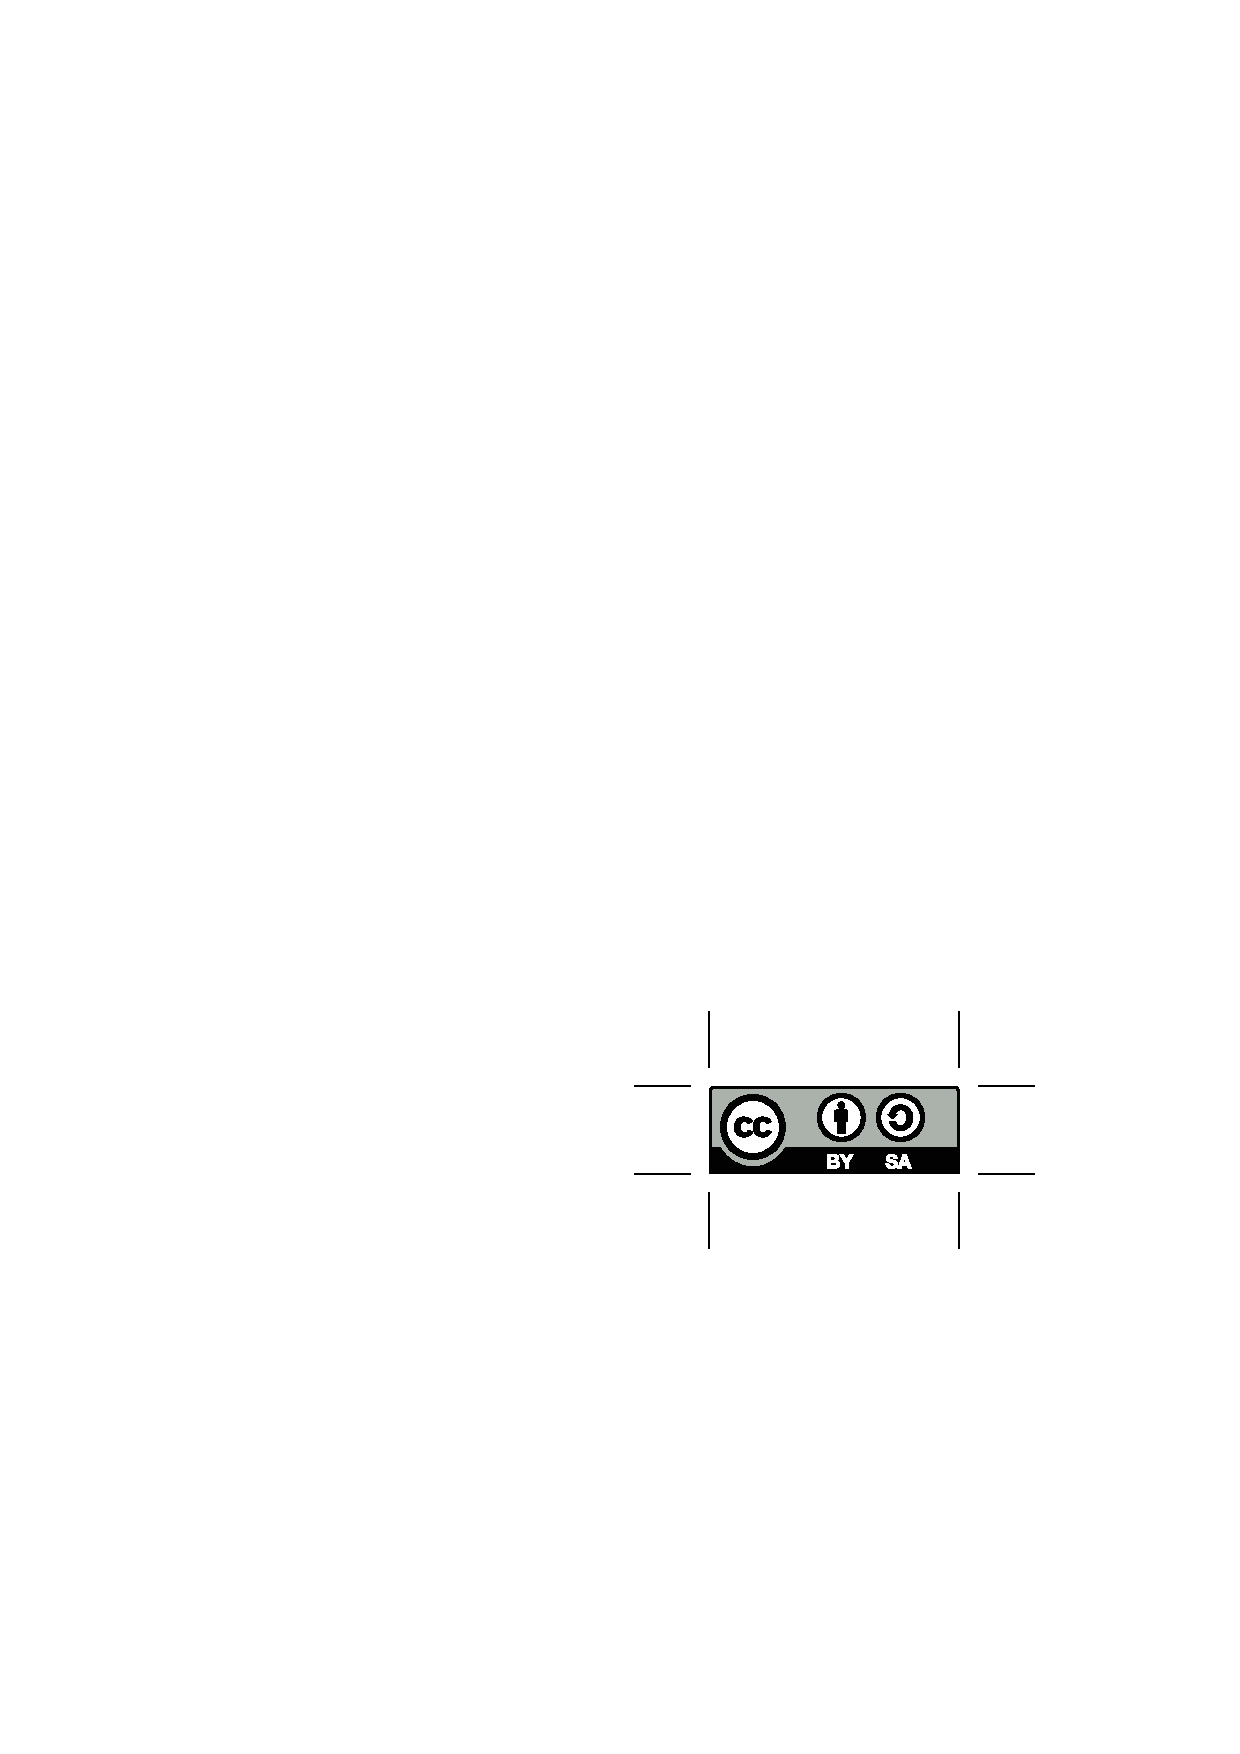
\includegraphics[scale=0.8]{cc}}

\end{document}
